\documentclass{beamer}
\usetheme{Warsaw}
\graphicspath{{figuras/}}
\setbeamercolor{normal text}{fg=white,bg=black!90}
\setbeamercolor{structure}{fg=white}

\setbeamercolor{alerted text}{fg=red!85!black}

\setbeamercolor{item projected}{use=item,fg=black,bg=item.fg!35}

\setbeamercolor*{palette primary}{use=structure,fg=structure.fg}
\setbeamercolor*{palette secondary}{use=structure,fg=structure.fg!95!black}
\setbeamercolor*{palette tertiary}{use=structure,fg=structure.fg!90!black}
\setbeamercolor*{palette quaternary}{use=structure,fg=structure.fg!95!black,bg=black!80}

\setbeamercolor*{framesubtitle}{fg=white}

\setbeamercolor*{block title}{parent=structure,bg=black!60}
\setbeamercolor*{block body}{fg=black,bg=black!10}
\setbeamercolor*{block title alerted}{parent=alerted text,bg=black!15}
\setbeamercolor*{block title example}{parent=example text,bg=black!15}
\setbeamercolor{figure text}{fg=black}

\setbeamertemplate{headline}{}

\usepackage[brazil,spanish]{babel}
\usepackage[utf8]{inputenc}
\usepackage{color}
\usepackage{listings}
\usepackage{setspace}
\usepackage{graphicx}

%%%%%%%%%%%%%%%%%%%%%%%%%%%%%%%%%%%%%%%%%%%%%%%%



\title[Defensa de Memoria]{\bf An\'alisis de Im\'agenes a trav\'es de la Transformaci\'on de Box-Cox}
% Titre du diaporama

% Sous-titre optionnel

\author{Fabián Castellano Núñez}
% La commande \inst{...} Permet d'afficher l' affiliation de l'intervenant.
% Si il y a plusieurs intervenants: Marcel Dupont\inst{1}, Roger Durand\inst{2}
% Il suffit alors d'ajouter un autre institut sur le modèle ci-dessous.

\institute[Universidad Técnica Federico Santa María]
  {
  Profesor Guia: Ronny Vallejos A.
  }


\date{Marzo,  2024}
% Optionnel. La date, généralement celle du jour de la conférence

\subject{Transformación BoxCox}
% C'est utilisé dans les métadonnes du PDF
\titlegraphic{
    
\includegraphics[width=3cm,keepaspectratio]{logo_dmat.png}%
    \hfill%
    
\includegraphics[width=2cm,keepaspectratio]{logo_usm3.png}%
}
%%%%%%%%%%%%%%%%%%%%%%%%%%%%%%%%%%%%%%%%%%%%%%%%%%%%%%%%%%%%%%%%%%%%%
\begin{document}

\begin{frame}
  \titlepage
\end{frame}

\begin{frame}{Contenidos}
  \tableofcontents
  % possibilité d'ajouter l'option [pausesections]
\end{frame}


\begin{frame}{Introducción}
    \begin{center}
        \begin{itemize}
            \item La transformación Box-Cox es una transformación de datos que es utilizada para estabilizar la varianza y hacer los datos más parecidos a una distribución normal.
            \item En este trabajo se propone utilizar la transformación Box-Cox para analizar imágenes.
            \item Se propone utilizar la transformación Box-Cox para encontrar el valor de $\lambda$ que maximiza la correlación entre imágenes.
        \end{itemize}
    \end{center}
\end{frame}



\section{Comparación entre imágenes}
\begin{frame}{Comparación entre imágenes}
\frametitle{Comparación entre imágenes}
\end{frame}

\subsection{Coeficiente de Información Máxima}
\begin{frame}{Coeficiente de Información Máxima}
     
    
    \begin{block}{Información mutua}
    Dada una distribución bivariada $P(x,y)$, definimos:
        \begin{equation}
            \mathrm{I}(X ; Y)=\int_{\mathcal{Y}} \int_{\mathcal{X}} P_{(X, Y)}(x, y) \log \left(\frac{P_{(X, Y)}(x, y)}{P_{X}(x) P_{Y}(y)}\right)dxdy
        \end{equation}
    \end{block}
     


    \begin{block}{Máximo sobre todas las mallas}
        Para un conjunto finito $D\in\mathcal{R}  ^2$ y enteros positivos $x,y$, definimos:
		$$
		I^*(D,x,y)=\max I(D|_G)
		$$
    \end{block}
    \begin{figure}
        \centering
        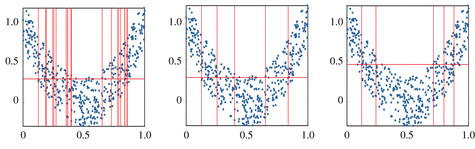
\includegraphics[scale=0.6] {rsos201424f03.png}
    \end{figure}
\end{frame}

\begin{frame}{Metodología: Coeficiente de Información Máxima}
    \begin{block}{Matriz Característica}
        Definimos la siguiente matriz       
        \begin{equation}
	    	M(D)_{x, y}=\frac{I^{*}(D, x, y)}{\log \min \{x, y\}}
        \end{equation}
        Notemos que en principio la matriz es infinita.
    \end{block}
     

    \begin{block}{Coeficiente de Información Máxima}
        Definido en por Reshef en 2011 \cite{reshef2011} Dado un conjunto de datos bivariado, tenemos:
        \begin{equation}
	    	\operatorname{MIC}(D)=\max _{x y<B(n)}\left\{M(D)_{x, y}\right\}
        \end{equation}
        donde $\omega(1)<B(n) \leq O\left(n^{1-\varepsilon}\right)$ para alg\'un $0<\varepsilon<1$. En el artiuclo utilizan $B(n)=n^{0.6}$
    \end{block}
\end{frame}

\subsection{Correlaci\'on y Covarianza por Distancia}

\begin{frame}{Correlaci\'on por Distancia}

    \begin{block}{Correlaci\'on por Distancia}
        Esta se Plantea como una generalizaci\'on de la correlaci\'on de Pearon, en particular cumple:
        \begin{enumerate}
            \item $\mathcal{R}(X,Y)$ est\'a definido para $X,Y$ de dimensi\'on aleatoria.
            \item $\mathcal{R}(X,Y) = 0$ caracteriza la independenc\'a de $X$ e $Y$.	 
        \end{enumerate}
    \end{block}

    \begin{block}{Correlaci\'on por Distancia}
        La Covarianza por distancia (dCov) entre los vectores aleatorios $X$ e $Y$ con primeros momentos finitos es el n\'umero no negativo $\mathcal{V}(X, Y)$ definido por:
        \begin{equation}
            \begin{aligned}\label{dcov_formula}
                \mathcal{V}^2(X, Y) & =\left\|f_{X, Y}(t, s)-f_X(t) f_Y(s)\right\|^2 \\
                & =\frac{1}{c_p c_q} \int_{\mathcal{R}^{p+q}} \frac{\left|f_{X, Y}(t, s)-f_X(t) f_Y(s)\right|^2}{|t|_p^{1+p}|s|_q^{1+q}} d t d s .
                \end{aligned}
        \end{equation}
    \end{block}
\end{frame}


\begin{frame}{Correlaci\'on por Distancia}
    \begin{block}{Varianza por distancia}
        Se define como la raiz cuadrada:

        $$
        \mathcal{V}^2(X)=\mathcal{V}^2(X, X)=\left\|f_{X, X}(t, s)-f_X(t) f_X(s)\right\|^2 .
        $$
    
        Por definici\'on de la norma $\|\cdot\|$, es claro que  $\mathcal{V}(X, Y) \geq 0$ y $\mathcal{V}(X, Y)=0$ si y solo si $X$ e $Y$ son indepentes.
        
    \end{block}
    \begin{block}{Correlaci\'on por Distancia}
        La correlaci\'on por distancia (dCor) entre los vectores aleatorios $X$ e $Y$ con primer momento finito es el n\'unero no negtivo $\mathcal{R}(X, Y)$ definido por:
		$$
		\mathcal{R}^2(X, Y)= \begin{cases}\frac{\mathcal{V}^2(X, Y)}{\sqrt{\mathcal{V}^2(X) \mathcal{V}^2(Y)}}, & \mathcal{V}^2(X) \mathcal{V}^2(Y)>0 \\ 0, & \mathcal{V}^2(X) \mathcal{V}^2(Y)=0\end{cases}.
		$$
    \end{block}
\end{frame}


\section{Análisis y Procesamiento de Imágenes}
\begin{frame}{Imágen cómo Matriz}
     
    \begin{block}{Imágen cómo Matriz}
        Una imagen es una representaci\'on visual de un objeto, y se puede definir como una funci\'on bidimensional $f(x,y)$, como se muestra en la siguiente ecuaci\'on:

        $$
        f(x, y)=\left[\begin{array}{cccc}
        f(0,0) & f(0,1) & \cdots & f(0, N-1) \\
        f(1,0) & f(1,1) & \cdots & f(1, N-1) \\
        \vdots & \vdots & & \vdots \\
        f(M-1,0) & f(M-1,1) & \cdots & f(M-1, N-1)
        \end{array}\right]
        $$
    \end{block}
\end{frame}

\begin{frame}{Imágen cómo Matriz}
    \begin{figure}[H]
        \centering
        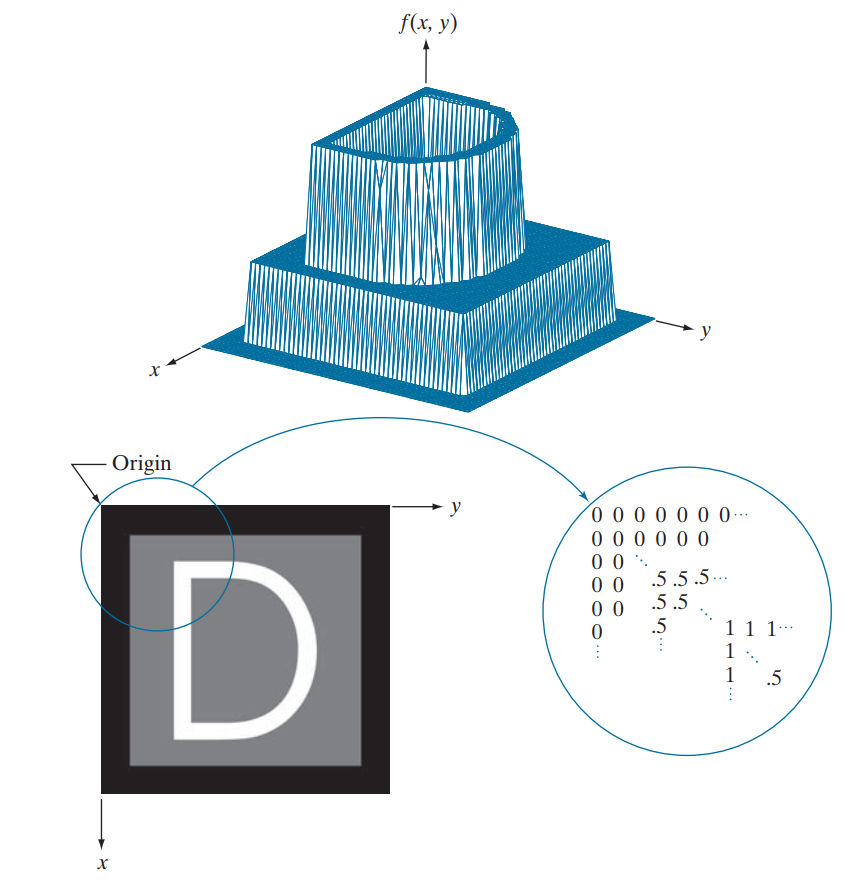
\includegraphics[width=0.5\textwidth]{dip_4_fig2_18.png}
    \end{figure}        
    (a) Como una superficie.
    (b) Como un conjunto de intensidades visuales.
    (c) Como un conjunto numérico en 2D.
\end{frame}

\begin{frame}{Imágen cómo Matriz}
    \begin{block}{Im\'agenes Escala de Grises}
        Nos interesa trabajar con escala de grises, lo hacemos de la siguiente forma.

        \begin{equation}
            I(x, y)=0.299 R(x, y)+0.687 G(x, y)+0.114 B(x, y), 
            \label{eq:grayscale}
        \end{equation}

        que corresponde el canal gris del espacio de colores $YC_bC_r$.
    \end{block}

    \begin{figure}[H]
        \centering
        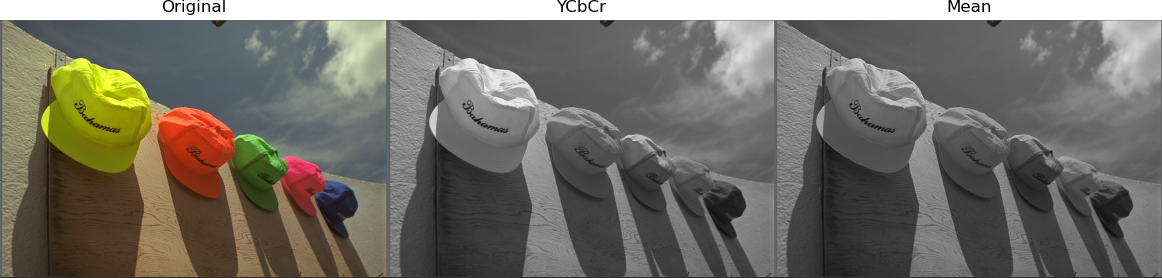
\includegraphics[width=0.8\textwidth]{img_ex_bw.png}
        \caption{Imagen RGB,escala de grises, y promedio simple.}
    \end{figure}
\end{frame}

\begin{frame}{Banco}
    \begin{figure}[H]
        \centering
        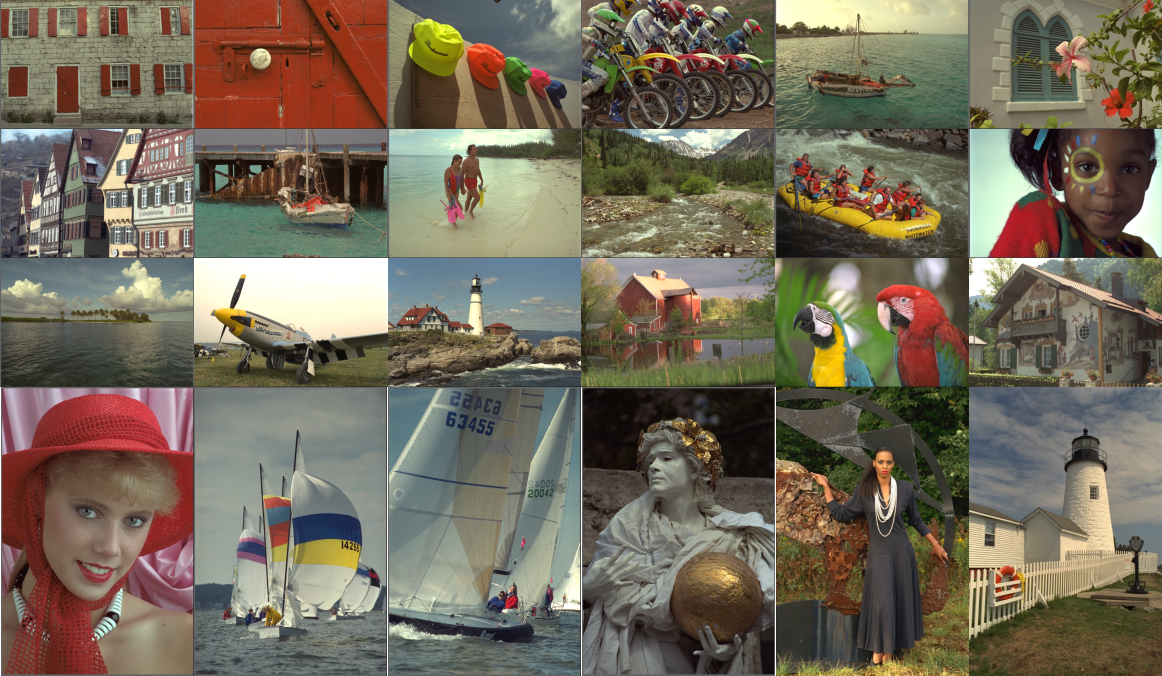
\includegraphics[width=0.8\textwidth]{all_images_grid.png}
        \caption{Banco de im\'agenes a utilizar.}
    \end{figure}        
\end{frame}

\begin{frame}{Correlaci\'on entre Im\'agenes}
    \begin{block}{Imagen a Vector}
        
    \end{block}

    \begin{block}{Histograma}
        
    \end{block}
    
\end{frame}

\begin{frame}{Ejemplos}
    \begin{figure}[H]
        \centering
        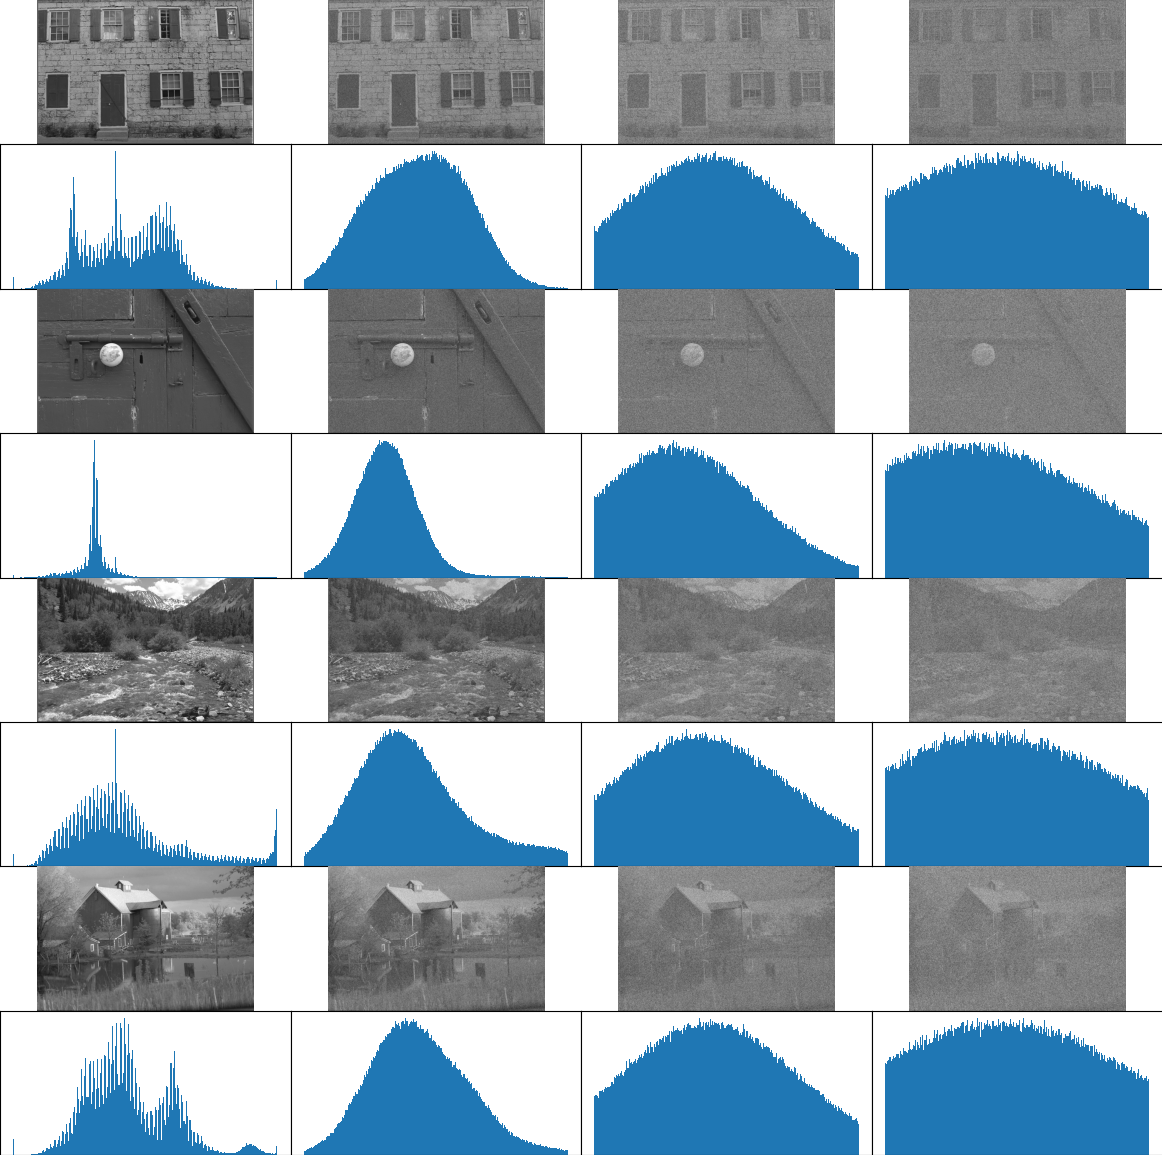
\includegraphics[width=0.6\textwidth]{img_hist_noise.png}
        \caption{im\'agenes junto con sus histogramas con ruido.}
        \label{fig:img_hist_ruido}
    \end{figure}
\end{frame}

\begin{frame}{Ejemplos}
    \begin{figure}[H]
        \centering
        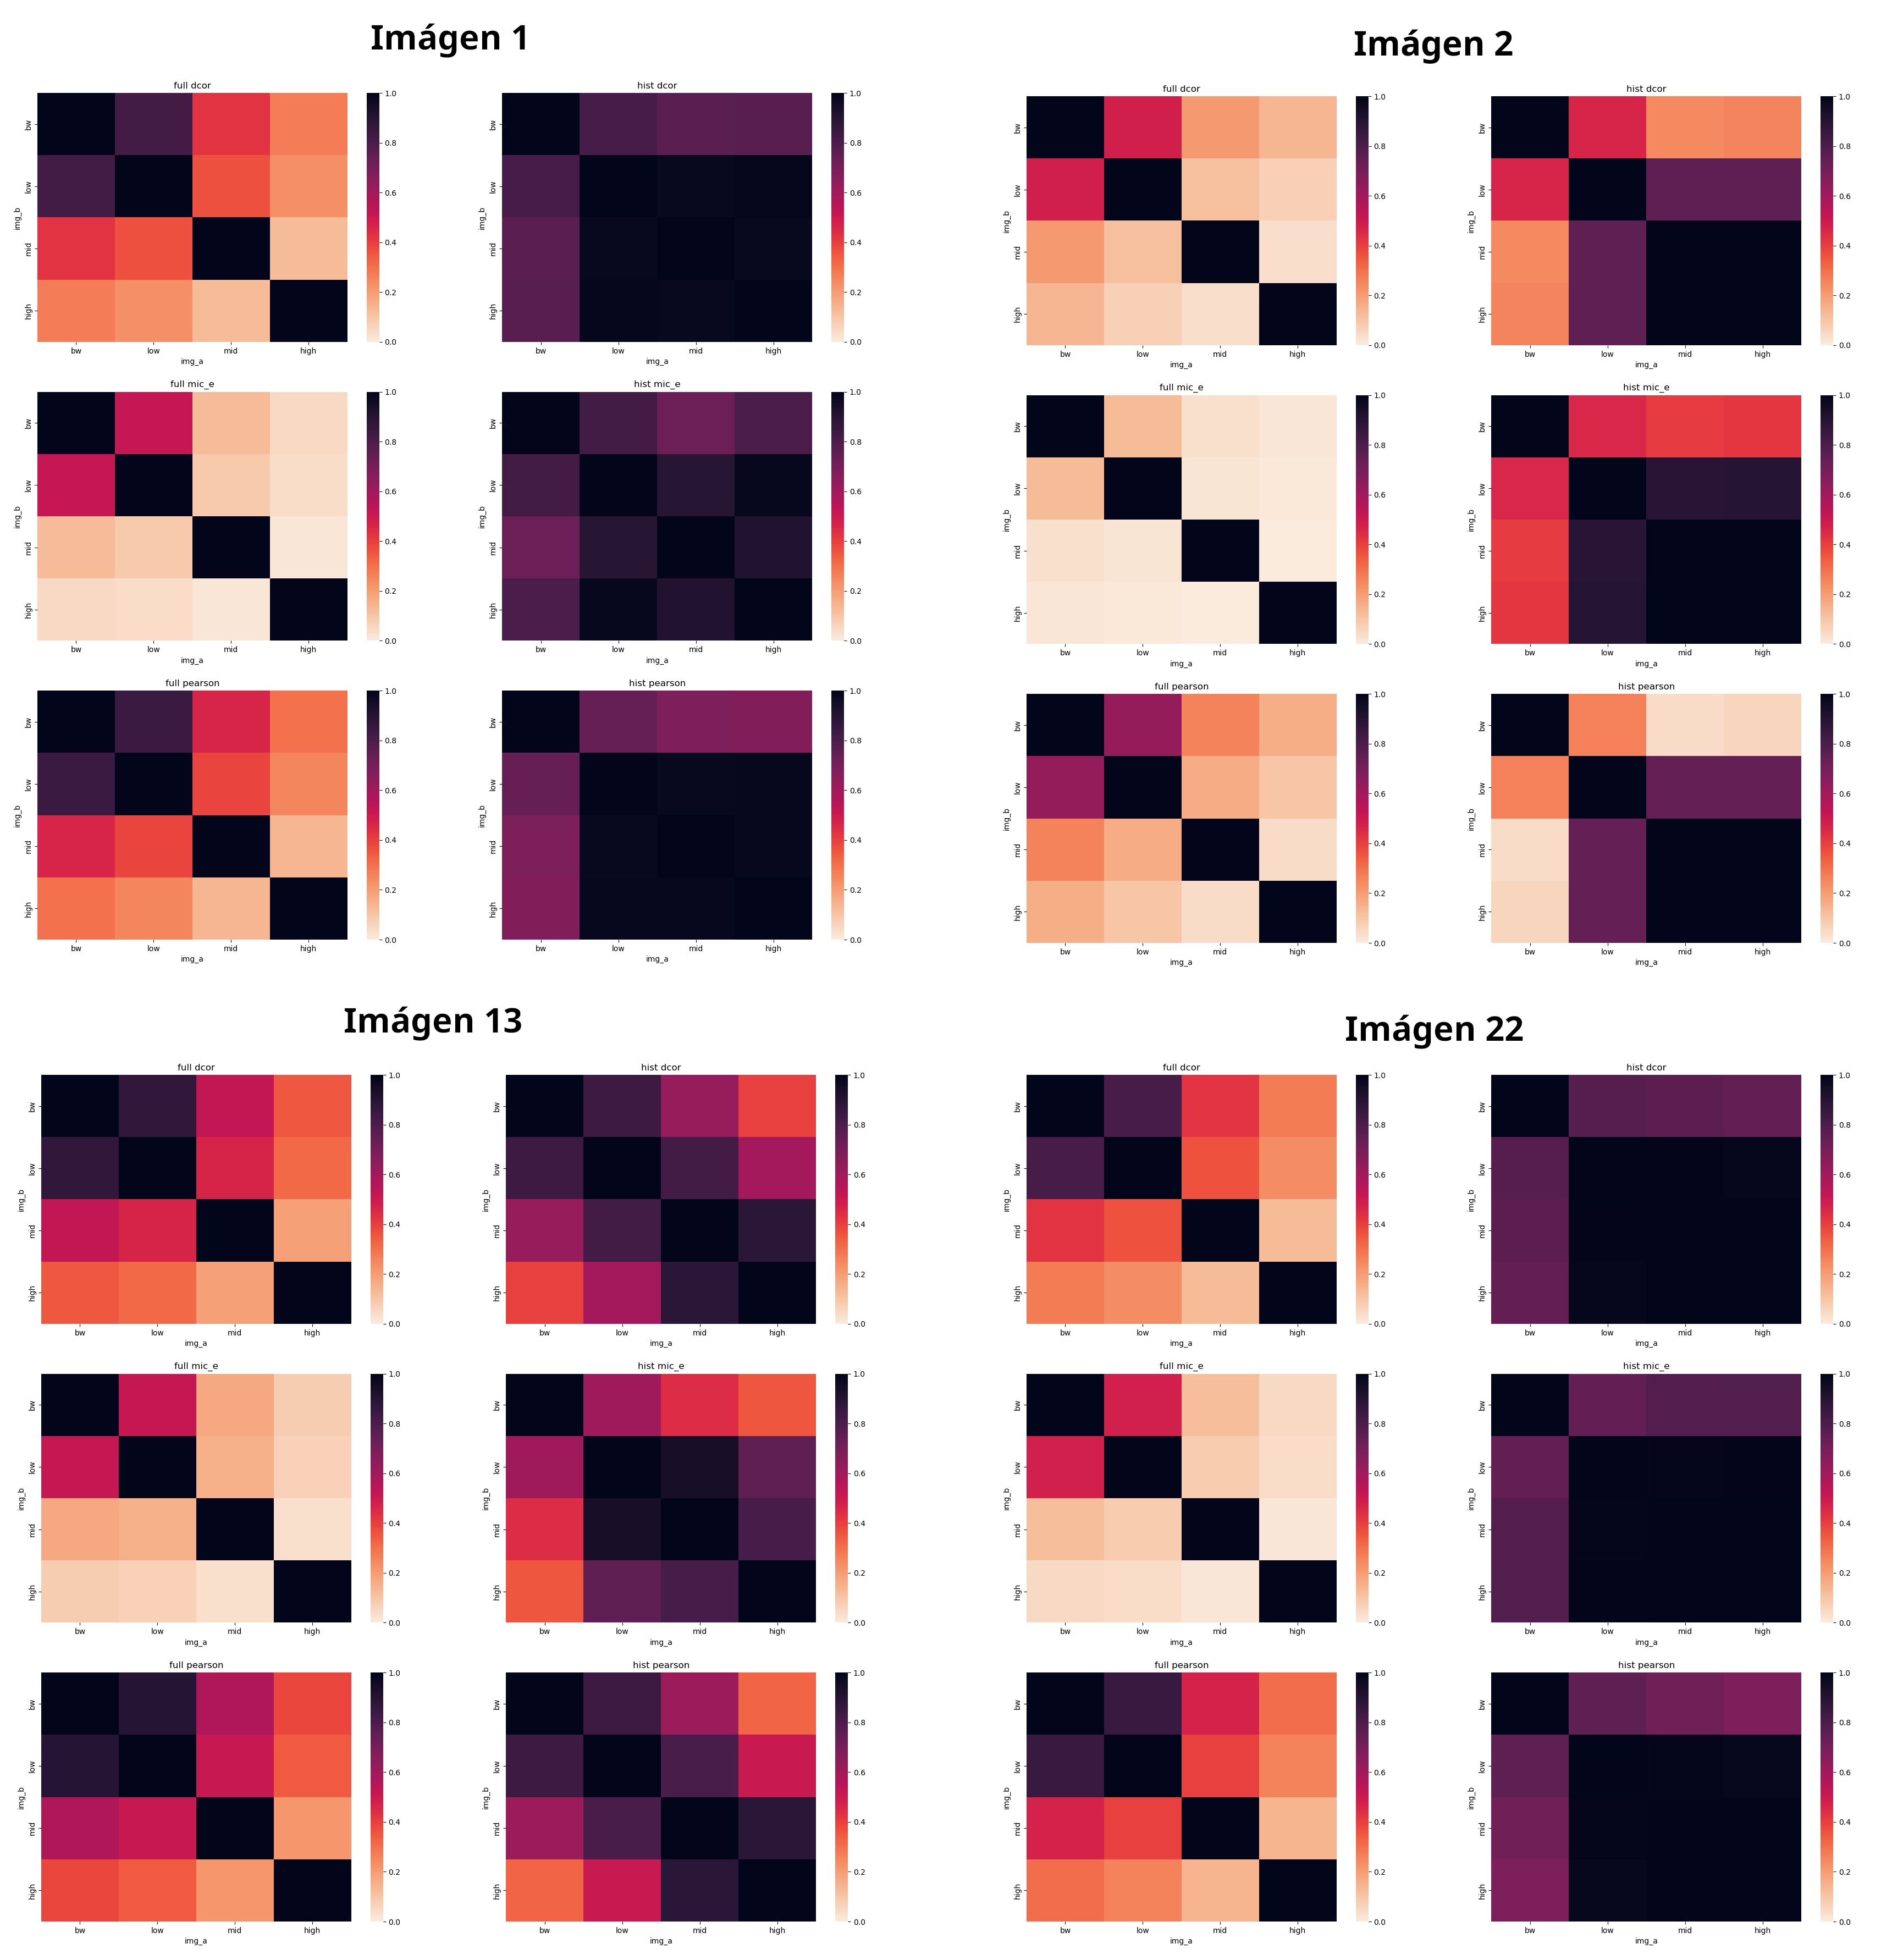
\includegraphics[width=\textwidth]{heatmap_all.png}
        \caption{Matriz de calor para las im\'agenes 1, 2, 13, y 22 del banco, cada mapa de calor corresponde a un m\'etodo de comparaci\'on, ya sea comparando el total de la imagen (izquierda), o el histograma de estas (derecha). La cantidad de ruido aumenta de izquierda a derecha, y de arriba hacía abajo.}
        \label{fig:heatmapall}
    \end{figure}
\end{frame}


\section{La transformación BoxCox}

\begin{frame}{La transformación BoxCox}
     
    \begin{block}{Transformación BoxCox}
    Como fue definida por Box y Cox en 1964 \cite{boxcox}
        \begin{equation}
            y^{(\lambda)}= \begin{cases}\frac{y^{\lambda}-1}{\lambda} & (\lambda \neq 0) \\ \log y & (\lambda=0)\end{cases}
        \end{equation}
    \end{block}
         
    \begin{block}{Verosimilitud}
        \begin{equation*}
            \mathcal{L}(\lambda) \equiv-\frac{n}{2} \log \left[\frac{1}{n} \sum_{j=1}^{n}\left(x_{j}^{\lambda}-\overline{x^{\lambda}}\right)^{2}\right] +(\lambda-1) \sum_{j=1}^{n} \log x_{j}
        \end{equation*}
    \end{block}
    
\end{frame}

\begin{frame}{Box-Cox en Imagenes}

    \begin{block}{Box-Cox para im\'agenes}
        Sea $\mathcal{F}^{\lambda_{\cdot}(x, y)}$ las im\'agen transformada para alg\'un $\lambda_\cdot$ seleccionado, entonces definimos BCI como:

    \begin{equation}
        BCI = \frac{\left(\mathcal{F}^{\lambda_{\cdot}}(x, y) - \min\left(\mathcal{F}^{\lambda_{\cdot}}(x, y)\right)\right)}{\left(\max\left(\mathcal{F}^{\lambda_{\cdot}}(x, y)\right) - \min\left(\mathcal{F}^{\lambda_{\cdot}}(x, y)\right)\right)}
    \end{equation}
        
        
    \end{block}
    
\end{frame}


\begin{frame}{Ejemplos}
    \begin{figure}
        \centering
        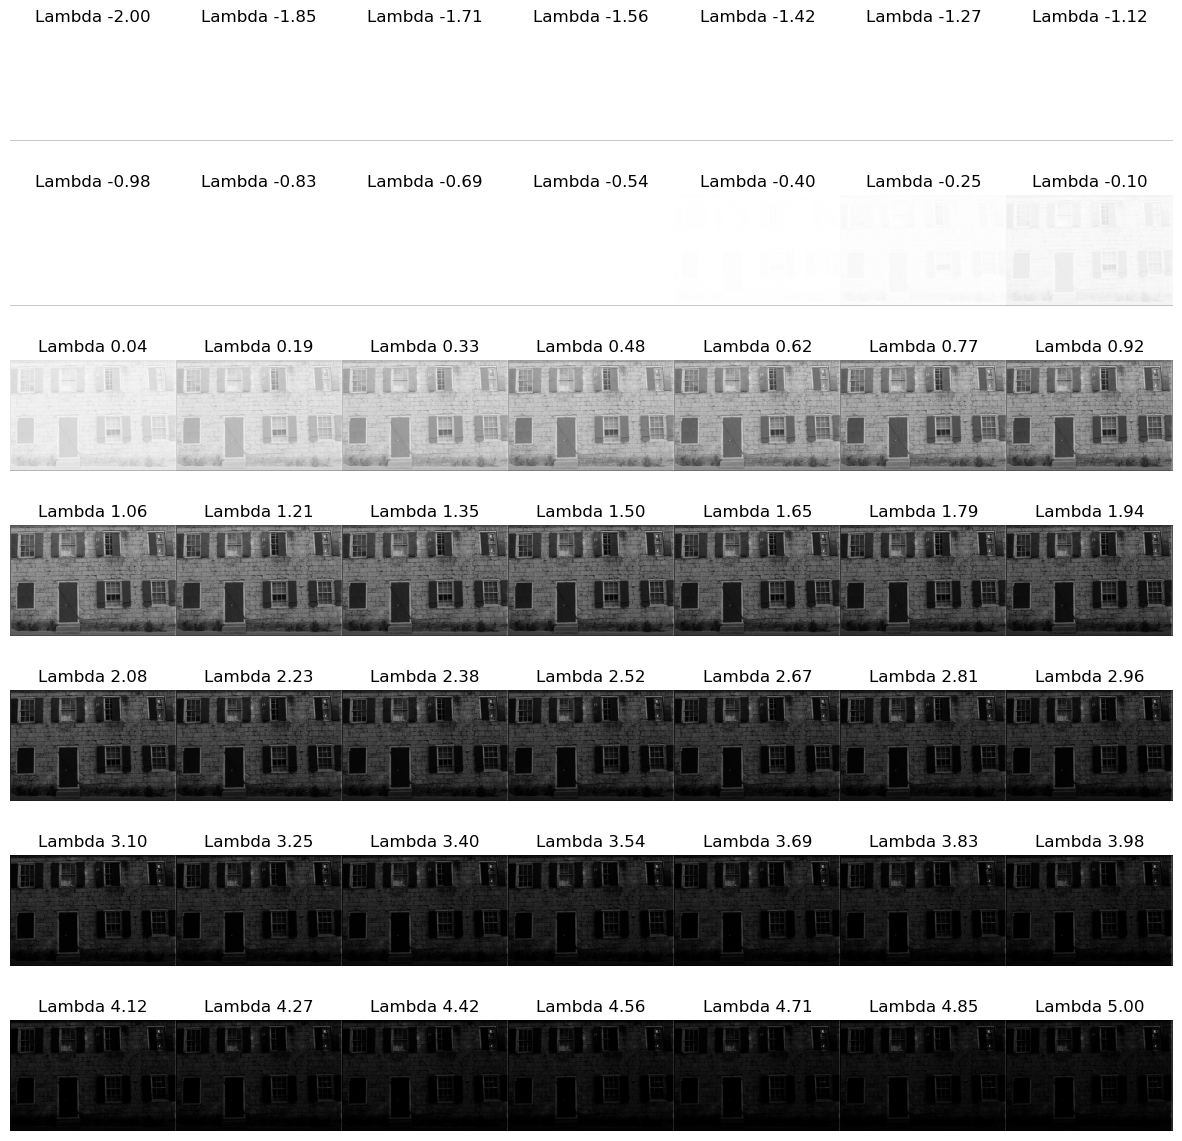
\includegraphics[width=0.6\textwidth]{all_lambda_1.png}
        \caption{Transformaciones de la im\'agen 1.}
        \label{fig:all_lambda_1}
    \end{figure}
\end{frame}


\begin{frame}{Ejemplos}

    \begin{figure}
        \centering
        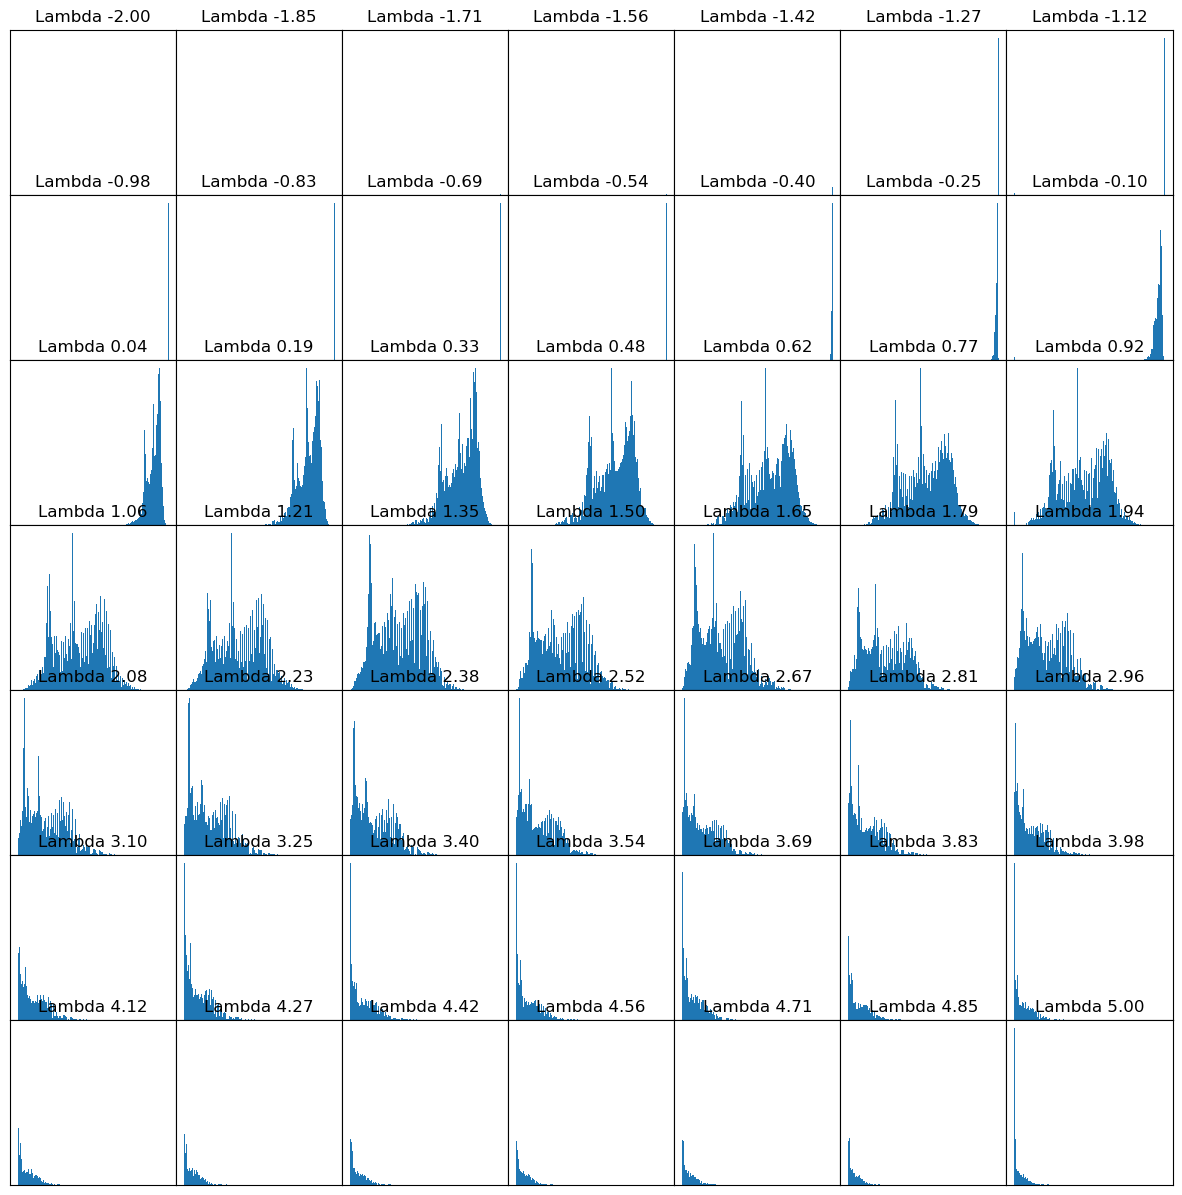
\includegraphics[width=0.6\textwidth]{all_lambda_hist_1.png}
        \caption{Histograma de las transformaciones de la im\'agen 1.}
        \label{fig:img_bci_hist_1}
    \end{figure}
\end{frame}



\begin{frame}{Ejemplos}

    \begin{figure}
        \centering
        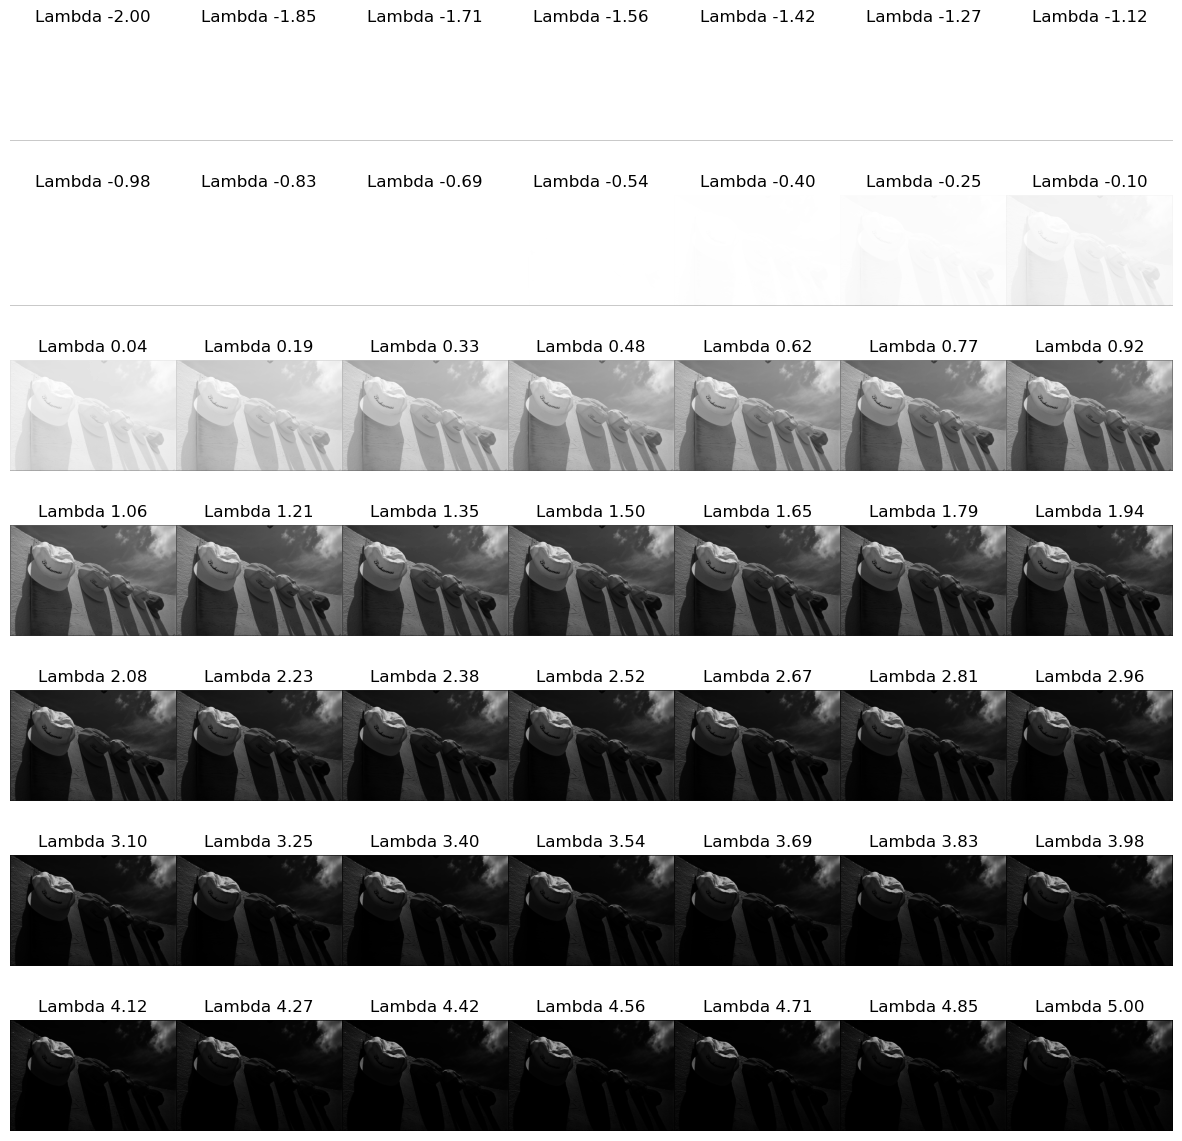
\includegraphics[width=0.6\textwidth]{all_lambda_3.png}
        \caption{Transformaciones de la im\'agen 3.}
        \label{fig:all_lambda_2}
    \end{figure}
\end{frame}

\begin{frame}{Ejemplos}

    \begin{figure}
        \centering
        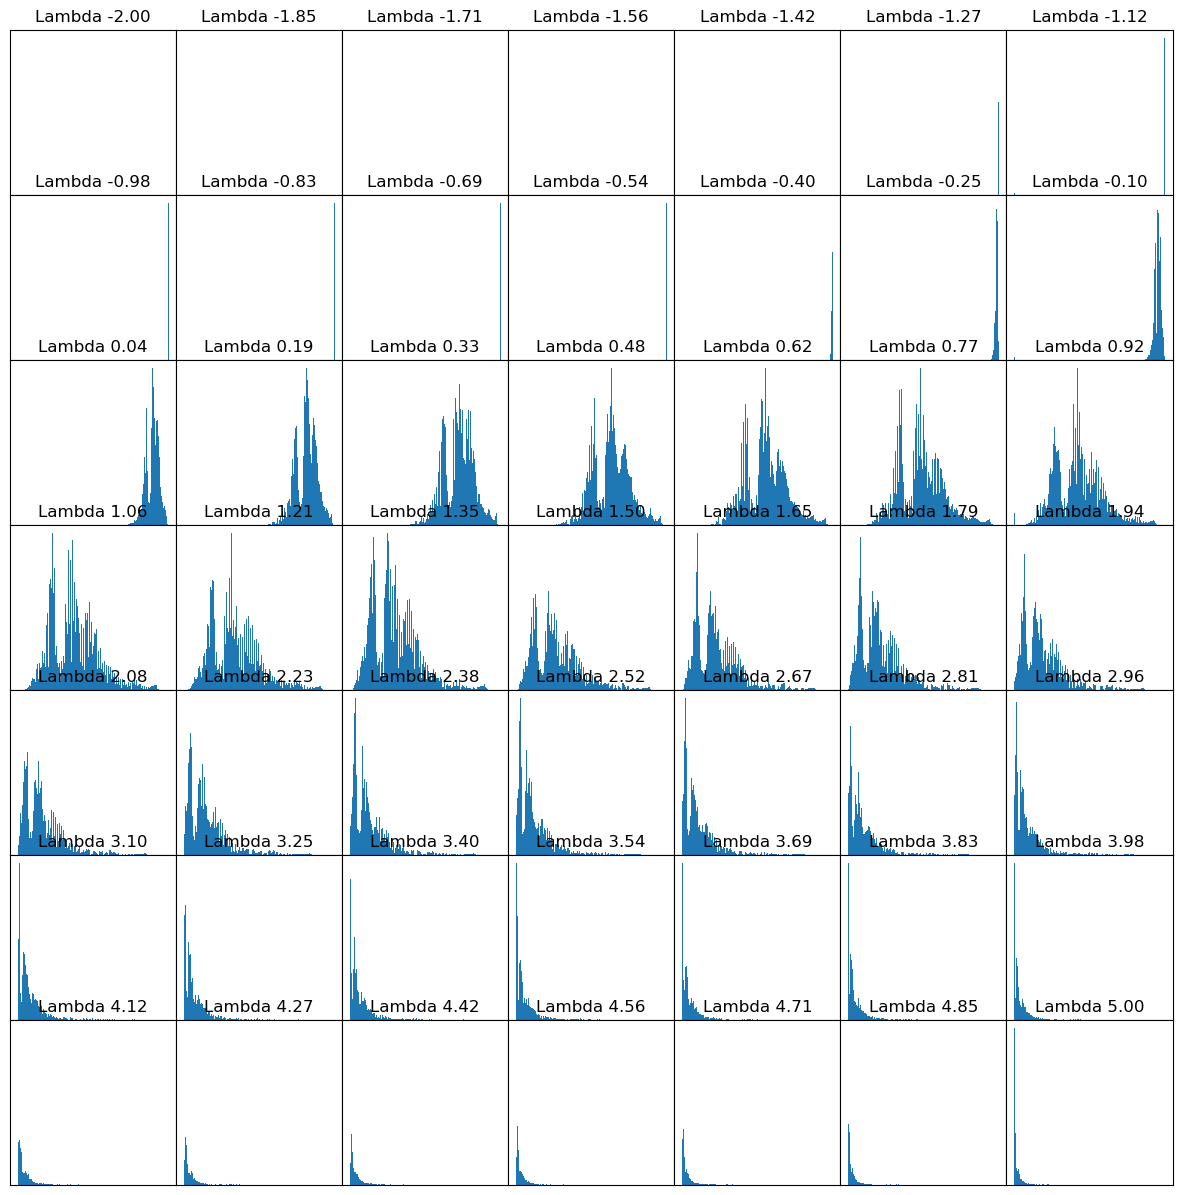
\includegraphics[width=0.6\textwidth]{all_lambda_hist_3.png}
        \caption{Histograma de las transformaciones de la im\'agen 2.}
        \label{fig:img_bci_hist_2}
    \end{figure}
\end{frame}

\begin{frame}{Seleccionando $\lambda$ en Im\'agenes}
     
    \begin{block}{Transformación 1-D}
        Transformar la imagen a un vector unidimensional, usar estos datos para determinar $\lambda$.
    \end{block}
    
         
    \begin{block}{Histograma}
        La idea es usar el histograma como un proxy comprimido de de la matriz de datos. 
    \end{block}
    
         
    \begin{block}{Grilla}
        La idea es usar una grilla sobre la imagen para mantener unformacion local al monento de encontrar $\lambda$
    \end{block}

\end{frame}

\begin{frame}{Ejemplos}
    \begin{figure}[H]
        \centering
        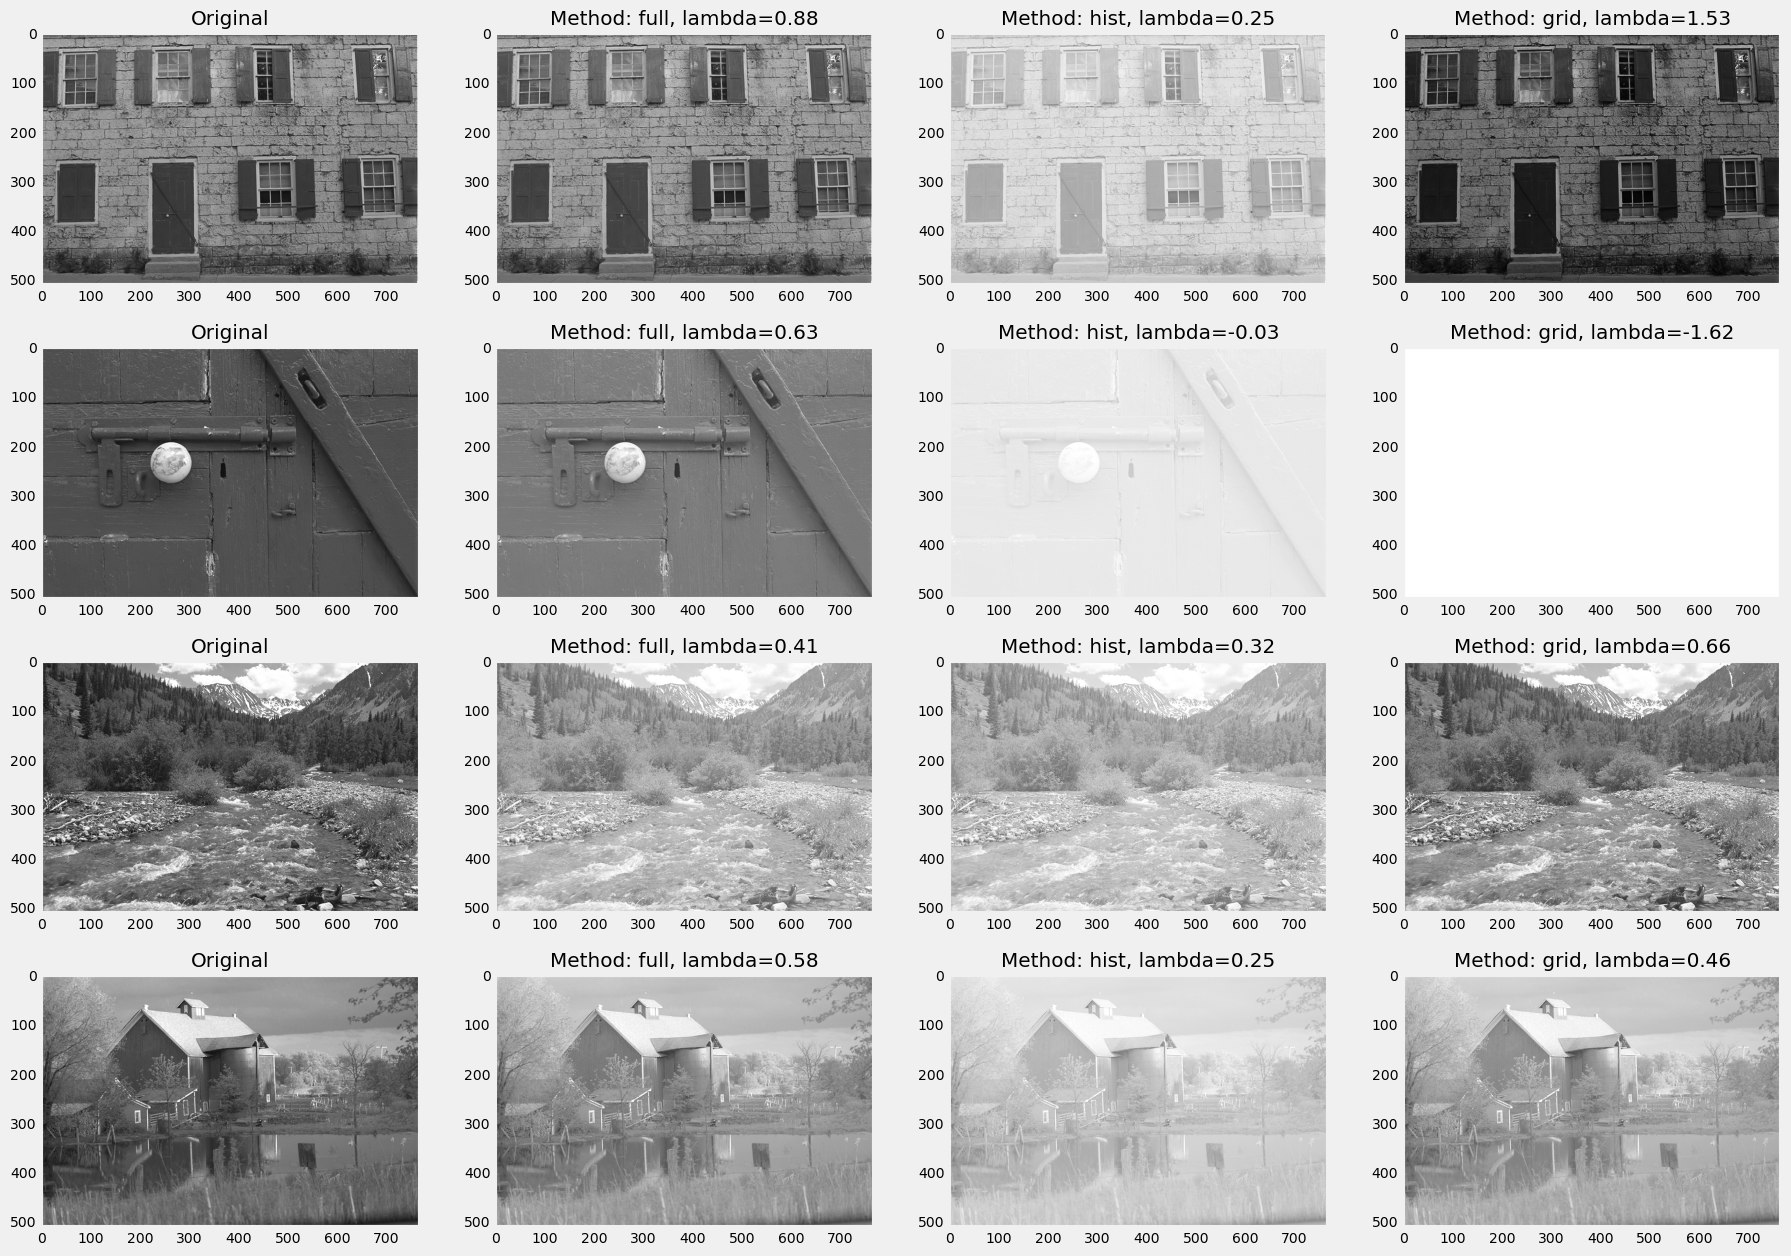
\includegraphics[width=0.7\textwidth]{img_bci_all.png}
        \caption{Transformaciones de la im\'agen 1, 2, 13, y 22. De izquierda a derecha, im\'agen original, m\'etodo de datos completos, m\'etodo de histograma, y m\'etodo de grilla.}
        \label{fig:img_bci_all}
    \end{figure}
\end{frame}

\begin{frame}{$\lambda$'s obtenidos}
    \begin{figure}[H]
        \centering
        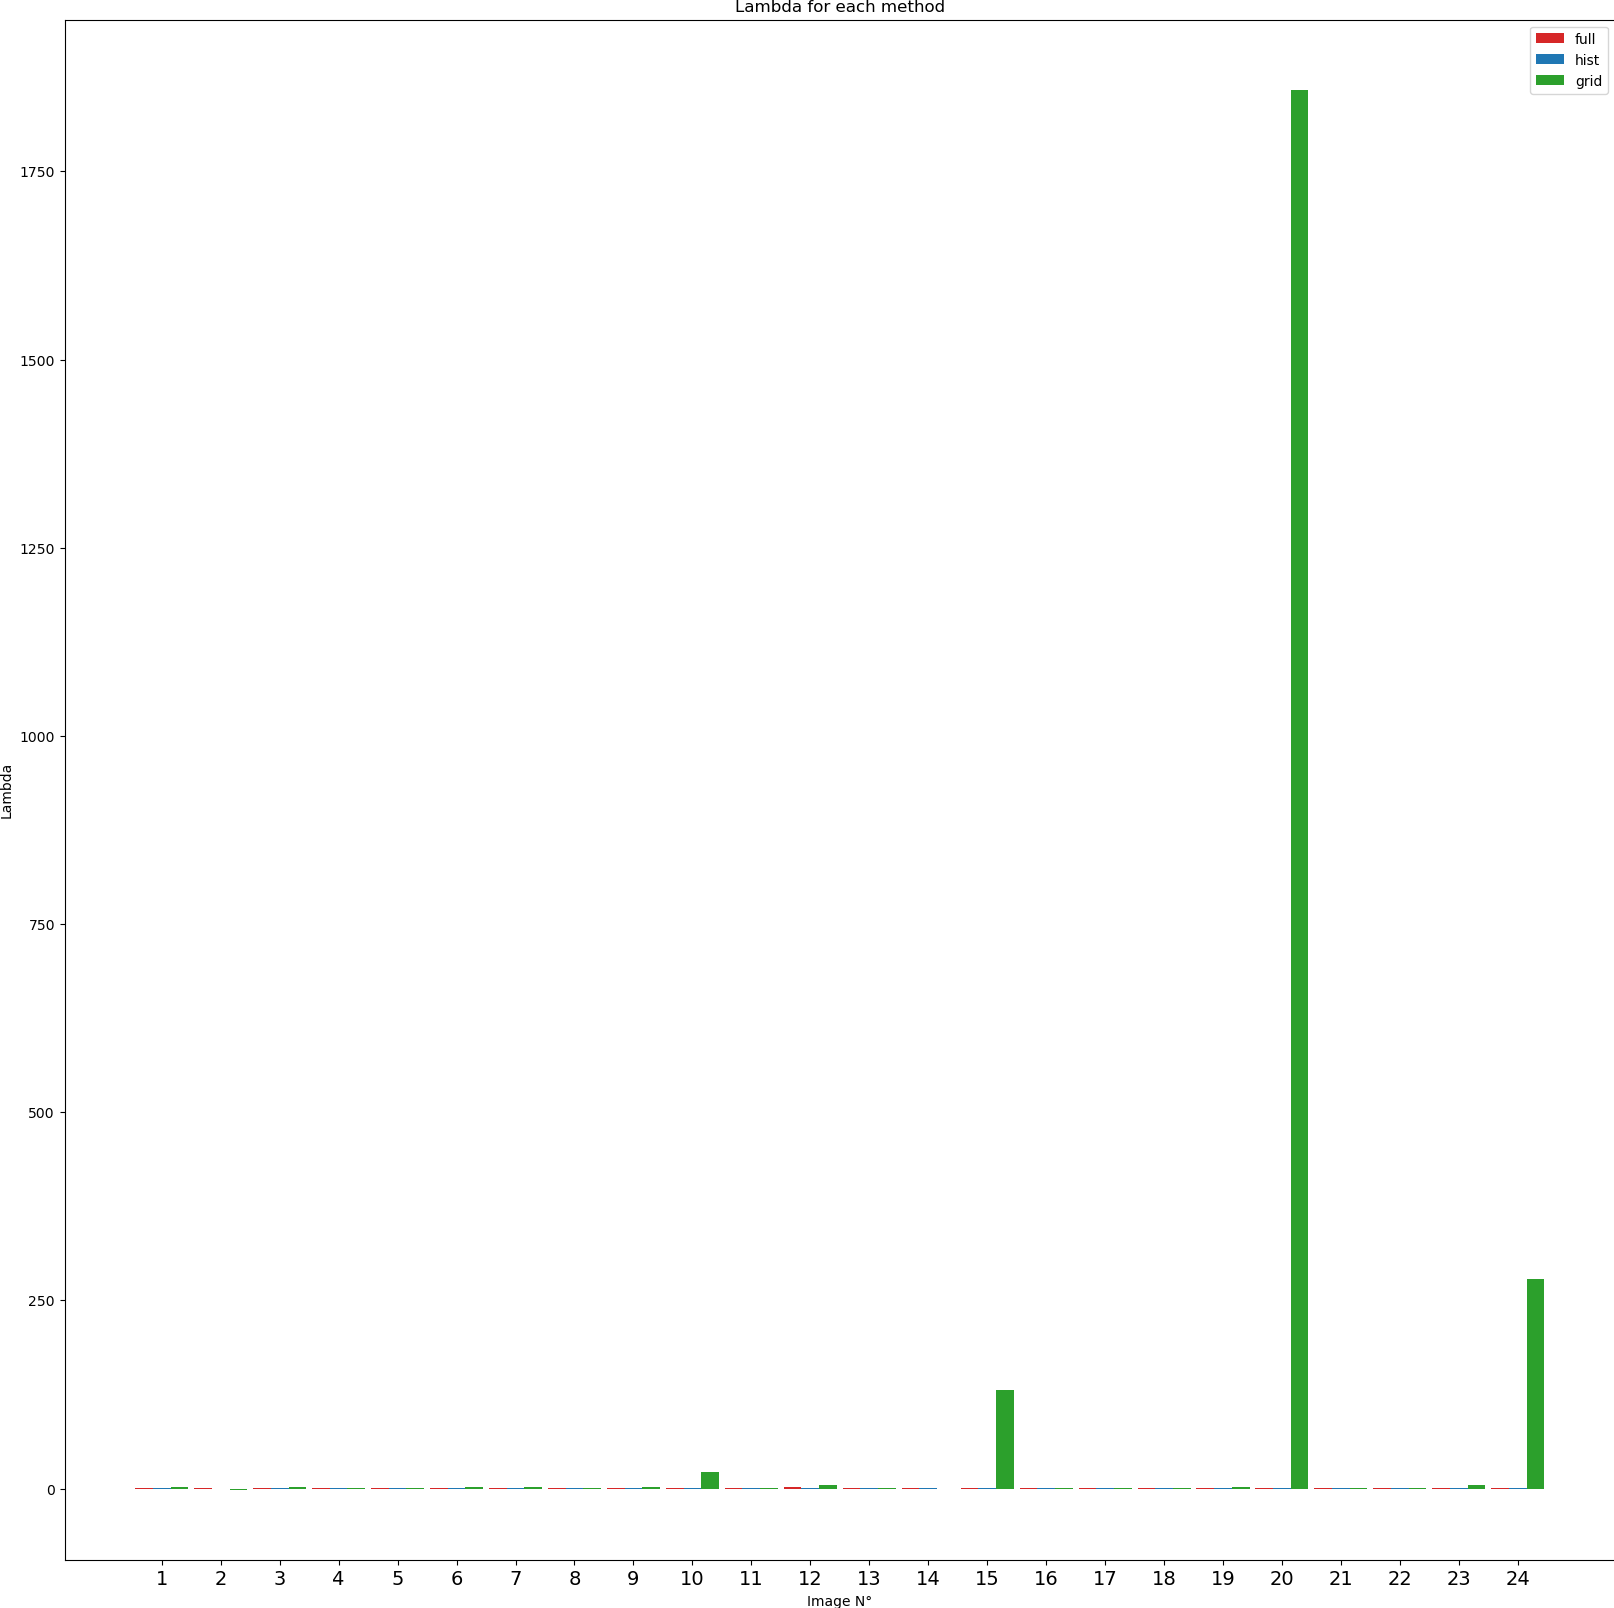
\includegraphics[width=0.6\textwidth]{lambda_noclip.png}
        \caption{Valores de $\lambda$ para todo el banco de im\'agenes. verde es el m\'etodo de grilla, azul es el m\'etodo de histograma, y rojo es el m\'etodo de datos completos.}
        \label{fig:lambda_noclip}
    \end{figure}

    \begin{figure}[H]
        \centering
        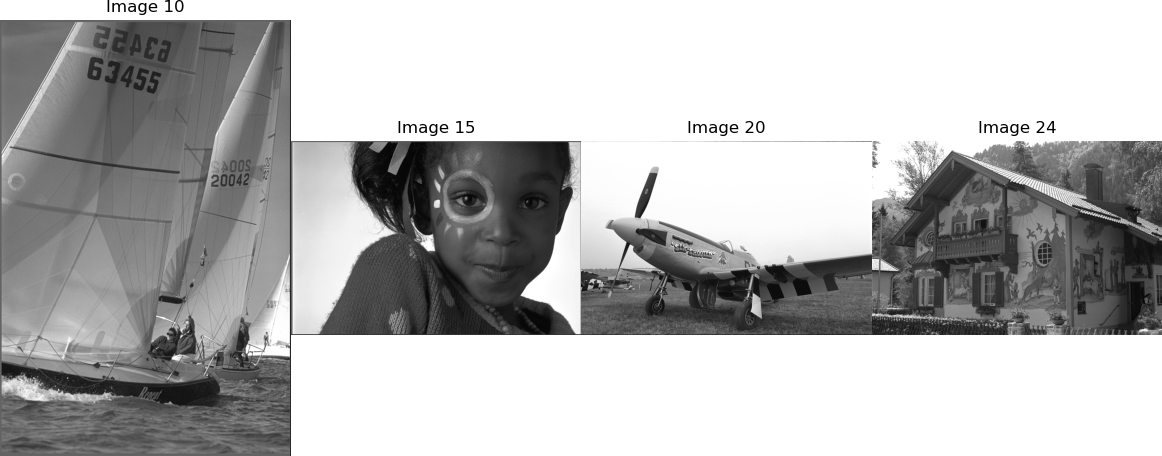
\includegraphics[width=0.9\textwidth]{img_ex_10_15_20_24.png}
        \caption{Transformaciones de las im\'agenes 10, 15, 20, y 24.}
        \label{fig:img_bci_10_15_20}
    \end{figure}

\end{frame}

\begin{frame}{$\lambda$'s obtenidos}
    \begin{figure}[H]
        \centering
        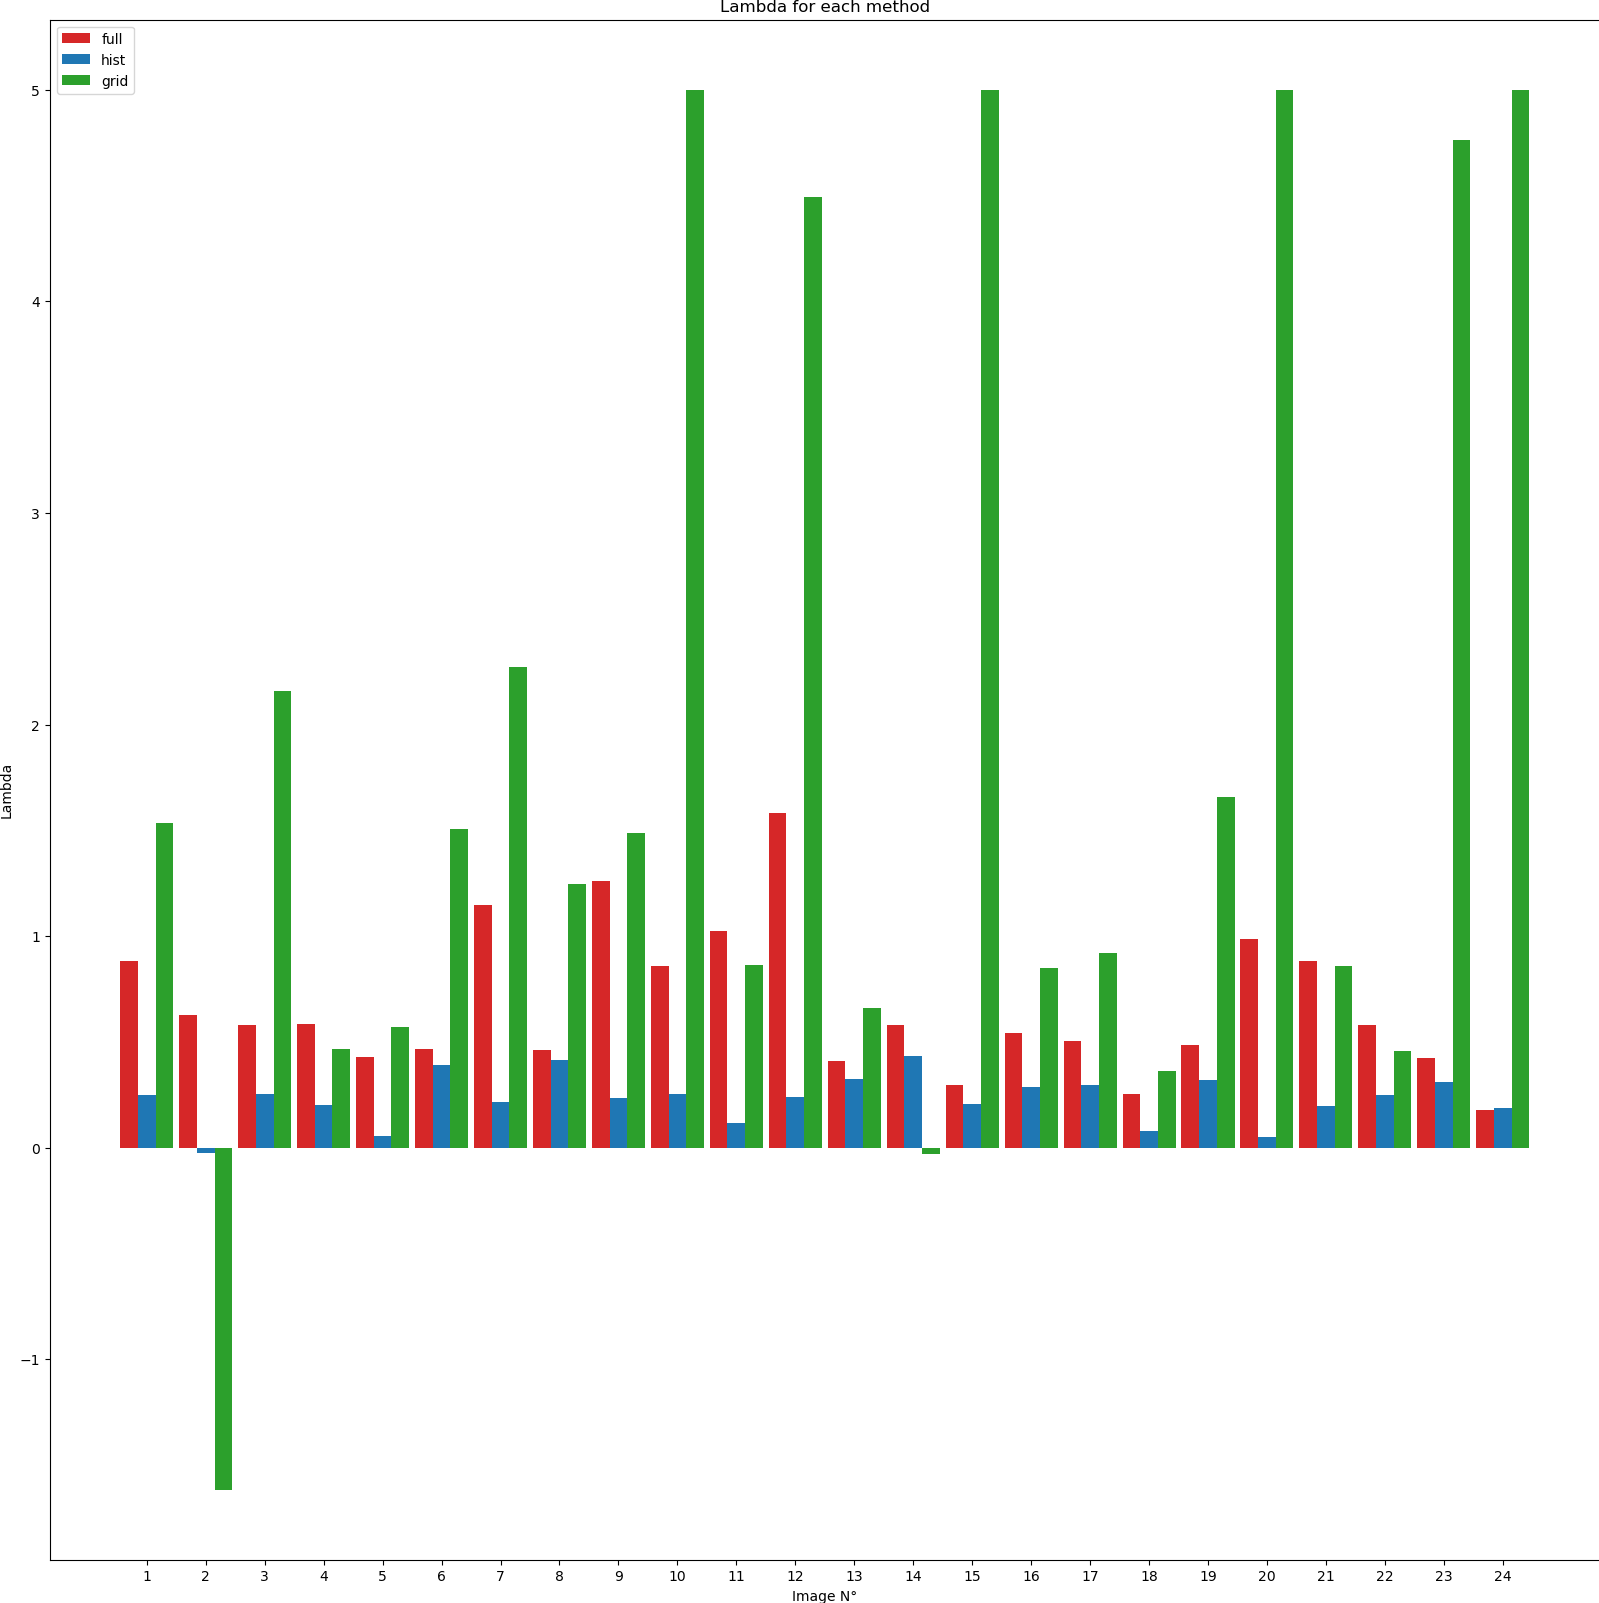
\includegraphics[width=0.5\textwidth]{lambda_clip.png}
        \caption{Valores de $\lambda$ para todo el banco de im\'agenes, cortado en 5. verde es el m\'etodo de grilla, azul es histograma, y rojo es datos completos}
        \label{fig:lambda_clip}
    \end{figure}
\end{frame}


\begin{frame}{Correlaciones}
    \begin{block}{Correlaciones}
        
        \begin{table}[H]
            \centering
            \begin{tabular}{|l|l|l|l|}
                \hline
                M\'etodo 1 & M\'etodo 2 & Pearson $\rho$ & Valor P \\ \hline
                Completo                  & Histograma                & -0.1305   & 0.5431  \\ 
                Completo                  & Grilla                    & 0.1384    & 0.5191  \\ 
                Histograma                & Grilla                    & -0.3467   & 0.0968  \\ \hline
            \end{tabular}
        \end{table}
    \end{block}
\end{frame}

\section{Experimentos}
\begin{frame}{Experimentos}
    \begin{figure}[H]
        \centering
        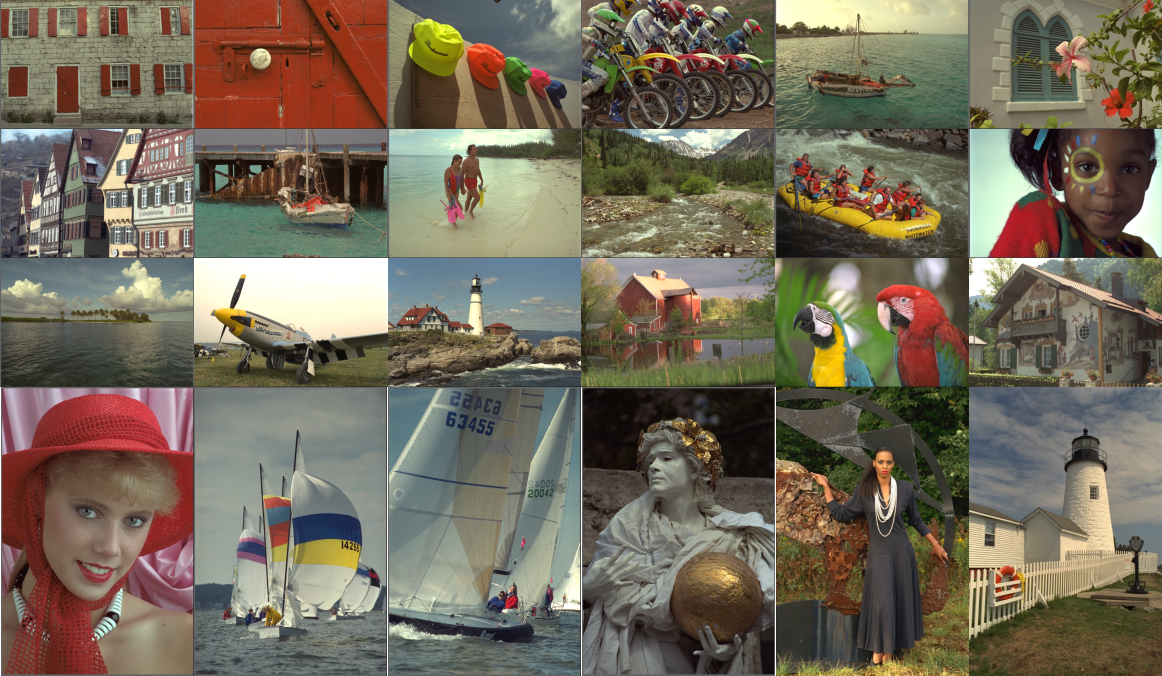
\includegraphics[width=0.8\textwidth]{all_images_grid.png}
        \caption{Banco de im\'agenes a utilizar.}
    \end{figure}        
\end{frame}

\begin{frame}{Experimentos}
    \begin{figure}[H]
        \centering
        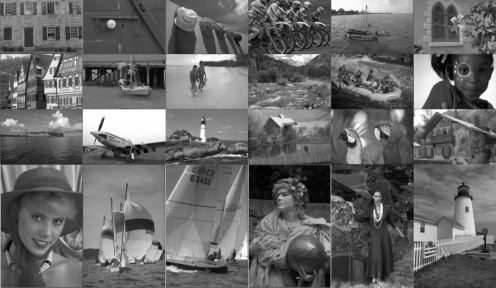
\includegraphics[width=0.8\textwidth]{all_images_grid_bw.png}
        \caption{Banco de im\'agenes a utilizar, en escala de grises.}
    \end{figure}     
\end{frame}

\begin{frame}{Experimentos}
    \begin{figure}[H]
        \centering
        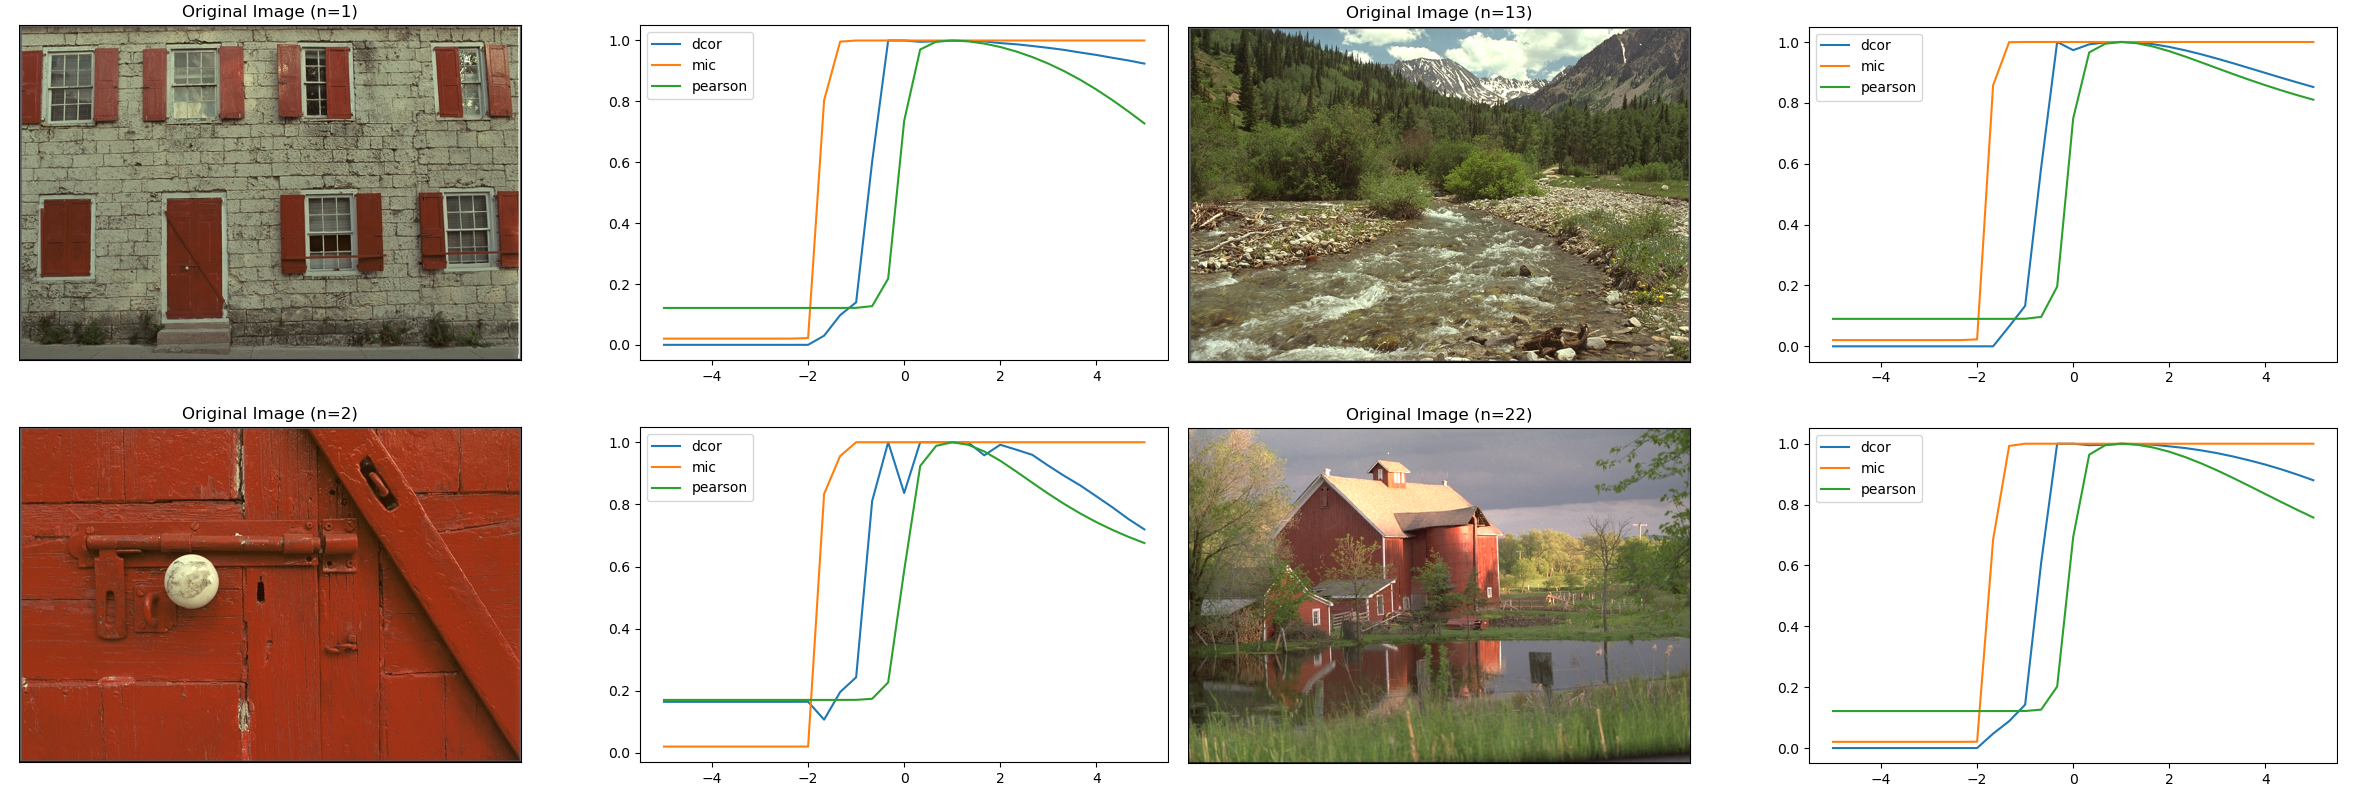
\includegraphics[width=\textwidth]{lam_v_com_all_img.png}
        \caption{De arriba hacia abajo, im\'agenes 1, 2, 13, y 22. A la izquierda la imagen original y a la derecha el valor de $dCor$ (azul), $MIC$ (naranja), y $\rho$ (verde) utilizando el vector completo en el eje y, $\lambda$ en el eje x.}
    \end{figure}
\end{frame}

\begin{frame}{Experimentos}
    \begin{figure}[H]
        \centering
        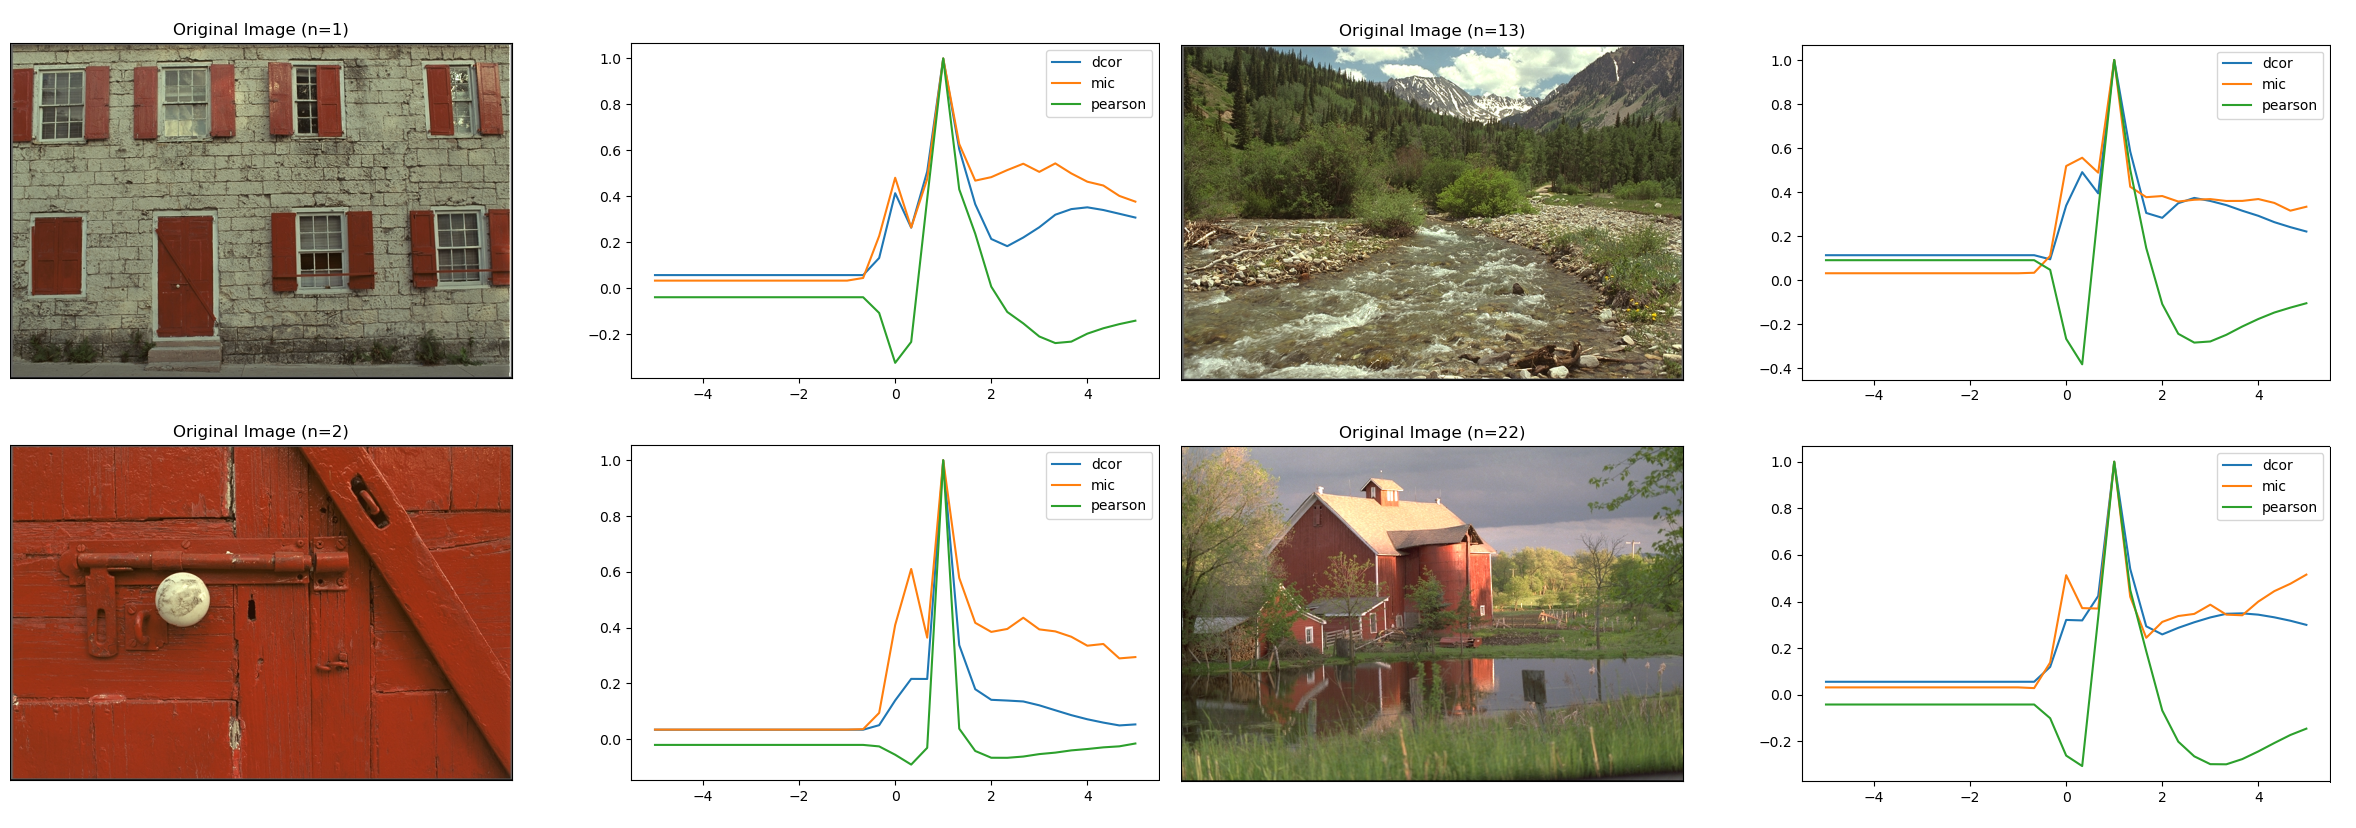
\includegraphics[width=\textwidth]{lam_v_com_all_img_hist.png}
        \caption{De arriba hacia abajo, im\'agenes 1, 2, 13, y 22. A la izquierda la imagen original y a la derecha el valor de $dCor$ (azul), $MIC$ (naranja), y $\rho$ (verde) utilizando el histograma en el eje y, $\lambda$ en el eje x.}
    \end{figure}
\end{frame}

\begin{frame}{Experimentos}
    \begin{figure}[H]
        \centering
        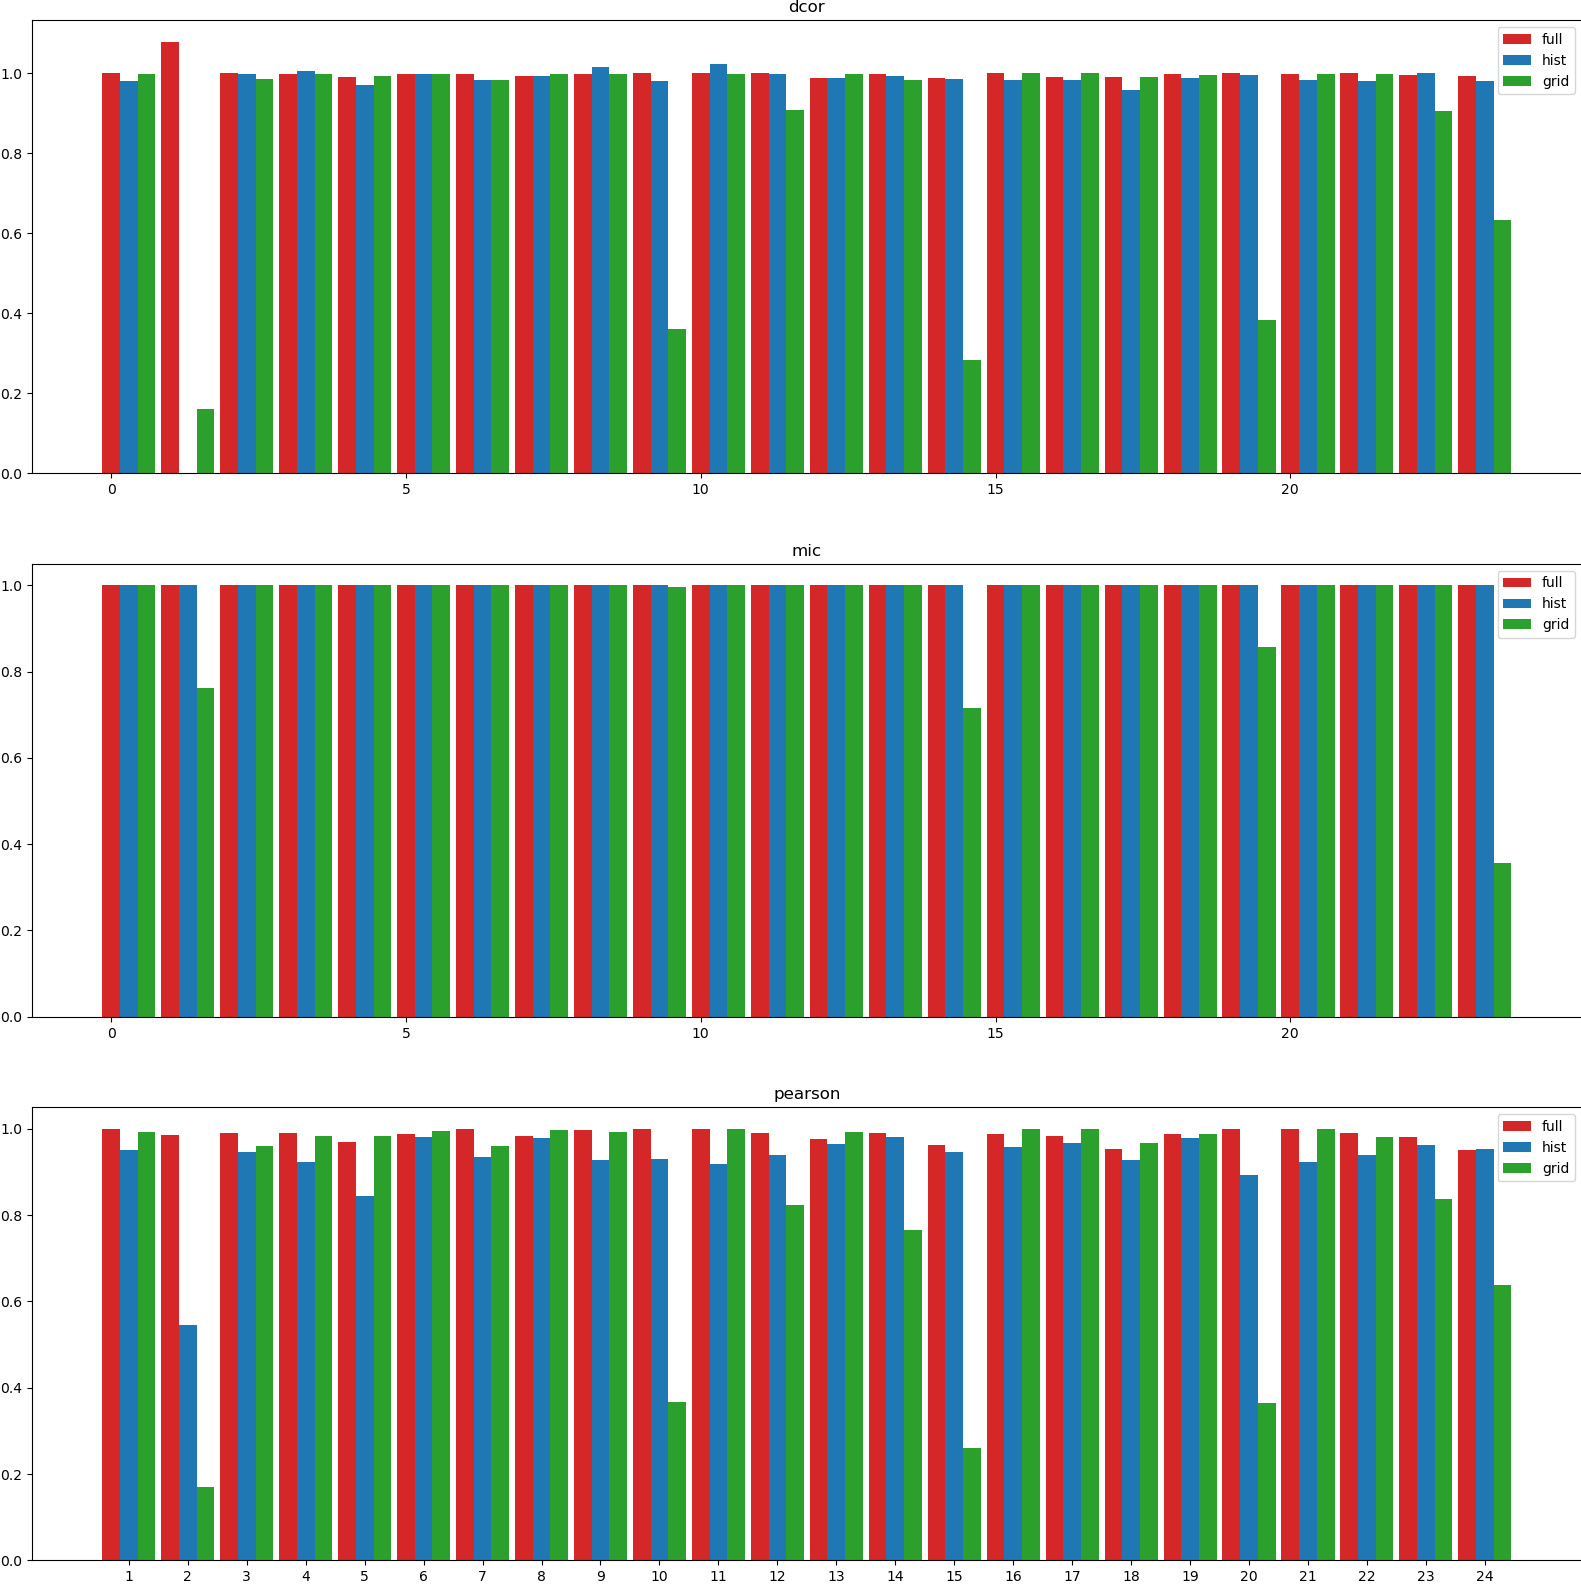
\includegraphics[width=0.6\textwidth]{plot_comparison_full.png}
        \caption{Valores de dcor, mic y pearson para cada imagen usando todo el vector, azul es el metodo para encontrar $\lambda$ con toda la imagen, rojo es el histograma y verde es el grilla.}
    \end{figure}
\end{frame}


\begin{frame}{Experimentos}
    \begin{figure}[H]
        \centering
        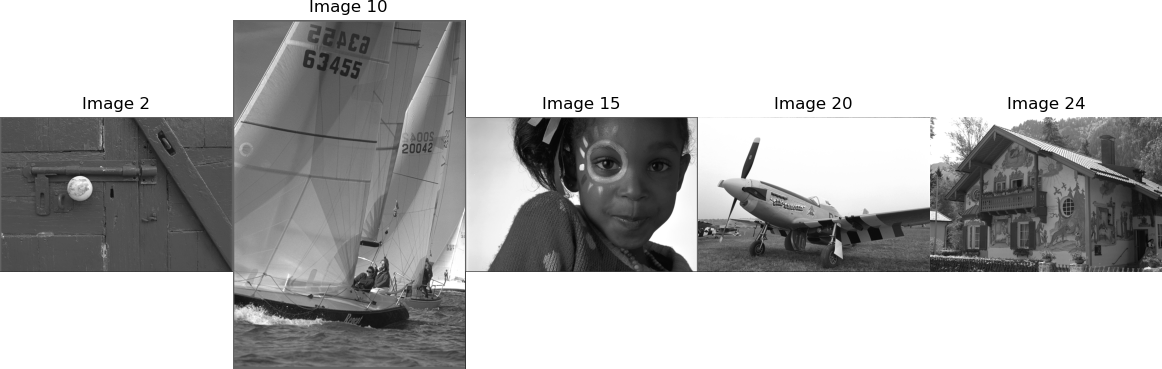
\includegraphics[width=\textwidth]{anomalies_grid.png}
        \caption{De izquierda a derecha, im\'agenes 2, 10, 15, 20, y 24 del banco.}
    \end{figure}
    Estos corresponden a los valores an\'omalos en el m\'etodo de grilla.
\end{frame}


\begin{frame}{Experimentos}
    \begin{figure}[H]
        \centering
        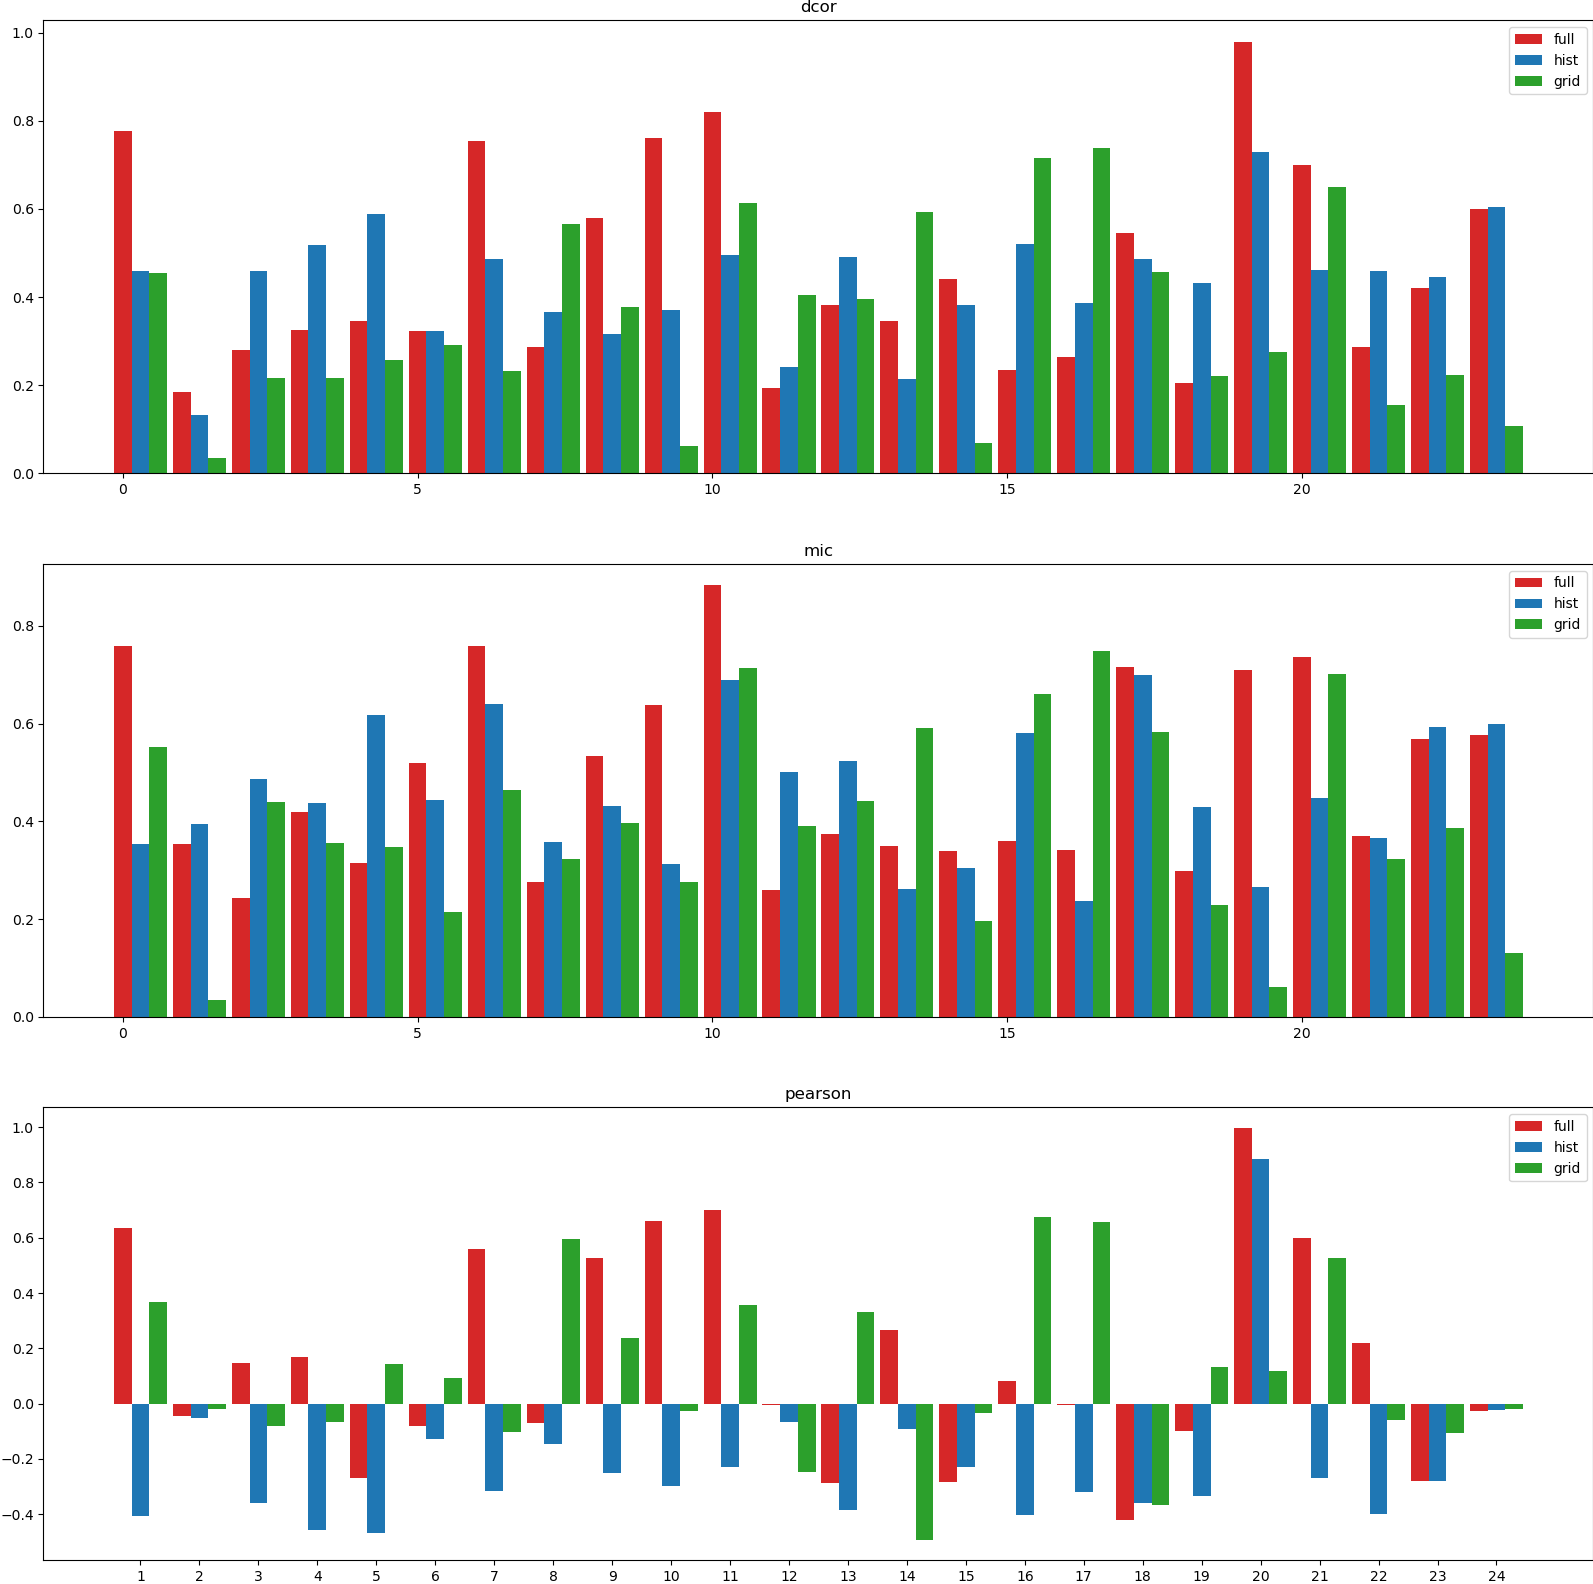
\includegraphics[width=0.6\textwidth]{plot_comparison_hist.png}
        \caption{Valores de dcor, mic y pearson para cada imagen usando el histograma, azul es el metodo para encontrar $\lambda$ con toda la imagen, rojo es el histograma y verde es el grid}
    \end{figure}
\end{frame}

\begin{frame}{Experimentos}
    \begin{block}{Corr.} 
        \begin{table}[H]
            \centering
            \begin{tabular}{|l|l|l|}\hline
            mic     & Completo    & 0.487  \\\hline
            dcor    & Completo    & 0.459  \\
            mic     & Histograma  & 0.457  \\
            dcor    & Histograma  & 0.431  \\
            mic     & Grilla      & 0.398  \\
            dcor    & Grilla      & 0.346 \\
            pearson & Completo    & 0.108  \\
            pearson & Grilla      & 0.108  \\
            pearson & Histograma  & -0.225 \\\hline
            \end{tabular}
        \end{table}
    \end{block}
\end{frame}

\section{Conlusiones}

\begin{frame}{Conlusiones}
    
    Muy concluido todo
\end{frame}


\begin{frame}{Bibliografía}
    \begin{thebibliography}{9}
    \bibitem{boxcox}
    Box, G. and Cox, D., 1964. An Analysis of Transformations. Journal of the Royal Statistical Society, 26(2), pp.211-252.
    
    \bibitem{chen2010}
    Chen, Y., Almeida, J., Richards, A., Müller, P., Carroll, R. and Rohrer, B., 2010. A Nonparametric Approach to Detect Nonlinear Correlation in Gene Expression. Journal of Computational and Graphical Statistics, 19(3), pp.552-568.
    
    \bibitem[]{reshef2011}
    Reshef, D., Reshef, Y., Finucane, H., Grossman, S., McVean, G., Turnbaugh, P., Lander, E., Mitzenmacher, M. and Sabeti, P., 2011. Detecting Novel Associations in Large Data Sets. Science, 334(6062), pp.1518-1524.
    
    \end{thebibliography}
\end{frame}

\begin{frame}{Bibliografía}
    \begin{thebibliography}{9}
    \bibitem[]{cheddad2020}
    Cheddad, A., 2020. On Box-Cox Transformation for Image Normality and Pattern Classification. IEEE Access, 8, pp.154975-154983.
    
    \bibitem[]{juin2009}
    Juin-Der Lee, Hong-Ren Su, Cheng, P., Liou, M., Aston, J., Tsai, A. and Cheng-Yu Chen, 2009. MR Image Segmentation Using a Power Transformation Approach. IEEE Transactions on Medical Imaging, 28(6), pp.894-905.
    
    \end{thebibliography}
\end{frame}
\end{document}




